\documentclass{fisatprojectfinal}
\renewcommand{\baselinestretch}{1.25} 
\usepackage{setspace}
\usepackage{tabularx}
\usepackage{booktabs}
\usepackage{float}
 \usepackage[utf8]{inputenc}
 \usepackage{xcolor}
 \usepackage{ragged2e}
 \usepackage{graphicx}

 \newcolumntype{L}{>{\RaggedRight\arraybackslash}X}
\title{CausalMedFusion: A Multimodal Causal Framework
for Chest Radiology Analysis}
\team{Anuroop P V}
\author{Anuroop P V}
\regno{FIT23CSD015}
\bibliographystyle{plain}

\begin{document}
	\maketitle
	\makecert
\newpage
\pagenumbering{roman}
\setcounter{page}{1}
\newgeometry{top=4cm,bottom=0.1cm}
\thispagestyle{empty}
\renewcommand\abstractname{ABSTRACT}
\begin{abstract}
	\vspace{2cm}
	\begin{onehalfspace}
		The integration of heterogeneous clinical data for predictive modeling in intensive care units (ICUs) remains a critical challenge in clinical artificial intelligence. Existing approaches typically process imaging, clinical text, laboratory measurements, and vital signs independently, overlooking their temporal interdependencies during patient progression.

This project introduces CausalMedFusion, a multimodal learning framework designed to model the temporal and causal evolution of patient state within the first 24 hours of ICU admission. The system structures raw multimodal inputs—including chest X-rays, clinical notes, laboratory data, and vital signs—into sequential time windows, enabling unified representation learning across modalities and time.

At the core of the framework is a Transformer-based architecture that performs intra-window multimodal fusion and inter-window temporal reasoning through causally constrained attention mechanisms. A two-stage training strategy is employed: first, the model learns clinically meaningful severity representations using a hybrid objective combining next-window prediction, intervention-aware supervision, and temporal discrimination; second, these representations are leveraged for downstream mortality prediction.

Preliminary results demonstrate that modeling temporally aligned multimodal interactions significantly improves the quality of learned patient representations and enhances predictive performance compared to modality-independent baselines. The proposed causal severity modeling framework provides improved interpretability by aligning intermediate representations with clinically meaningful progression.

This work contributes a novel approach to multimodal clinical modeling by explicitly incorporating temporal causality into representation learning. The resulting system has the potential to support early risk stratification and informed clinical decision-making, advancing the development of robust, real-time ICU decision support systems.
	\end{onehalfspace}
\end{abstract}
\newpage
\renewcommand\abstractname{Contribution by Author}
\thispagestyle{plain}
\begin{abstract}
	\vspace{1 cm}
	Author  Contribution:  
    \begin{itemize}
        \item Full frontend implementation: patient registration, visit management, multimodal
assessment upload, and results visualisation.

        \item System architecture design: full-stack integration of React frontend, Django REST
API, Celery/Redis task queue, FastAPI microservices, HDF5 and PostgreSQL storage
layers.
        \item Data pipeline development: four independent microservices for CXR embedding,
report embedding, vitals processing (30-minute binning, z-score normalisation), and
lab measurement extraction, all processing MIMIC-IV, MIMIC-CXR-JPG, and
MIMIC-IV-Note data.
        \item Deep learning model design and implementation: WindowEncoder (multi-head
Transformer), SeverityEncoder (causal block cross-attention), SeverityPooling, and
output heads for mortality and intervention prediction.
        \item Two-stage training loop: Stage 1 hybrid loss with EMA momentum encoder and
window order discriminator; Stage 2 mortality fine-tuning with frozen severity
representations.
        \item Model export: TorchScript tracing, ONNX export, and per-window isotonic calibration.

    \end{itemize}
    
	
	\vspace{1cm}
	\begin{flushright}
		Anuroop P V
	\end{flushright}
\end{abstract}

\newpage
\renewcommand\abstractname{ACKNOWLEDGMENT}
\thispagestyle{plain}
\begin{abstract}
	\vspace{1cm}
	I would like to express my sincere gratitude to Ms. Sheelu Susan Mathews, Project Guide, for
her invaluable guidance, constructive feedback, and encouragement throughout the
development of this project. \\
I am also grateful to Ms. Merin Cherian, Project Coordinator, for her administrative support
and for ensuring a smooth project review process. \\ 
I extend my thanks to Dr. Paul P Mathai, Head of the Department of Computer Science and
Engineering, FISAT, for providing an intellectually stimulating environment and the
resources necessary to undertake this work. \\
I am grateful to the research community behind the MIMIC family of datasets — MIMIC-IV,
MIMIC-CXR-JPG, and MIMIC-IV-Note — maintained by PhysioNet and the MIT
Laboratory for Computational Physiology, without which this project would not have been
possible. \\
Finally, I thank my family and friends for their unwavering support and patience throughout
this journey.
	\vspace{1cm}
	\begin{flushright}
		Anuroop P V
	\end{flushright}
\end{abstract}
\newpage

\thispagestyle{empty}

\restoregeometry

\newpage



\thispagestyle{empty}

\setcounter{page}{0}

\tableofcontents


\thispagestyle{empty}

\newpage


\cleardoublepage

\addcontentsline{toc}{chapter}{\listfigurename}

\thispagestyle{empty}

\pagenumbering{gobble}

\listoffigures

\thispagestyle{empty}

\newpage


\cleardoublepage

\addcontentsline{toc}{chapter}{\listtablename}


\thispagestyle{empty} % This line removes page numbers from the List of Tables

\pagenumbering{gobble}

\listoftables

\thispagestyle{empty}

\newpage

\chapter{Introduction}
\pagenumbering{arabic}
\setcounter{page}{1}
\renewcommand{\baselinestretch}{1.50}
\section{Overview}
Intensive care units (ICUs) generate diverse and continuous clinical data, including chest radiographs, clinical notes, vital signs, and laboratory measurements. Each modality reflects a different aspect of patient physiology, yet effective clinical decision-making depends on their joint interpretation over time. Clinicians naturally integrate these signals to assess patient condition, but most existing artificial intelligence models fail to replicate this process. \\

Current approaches are largely unimodal or rely on late fusion of independently learned representations, limiting their ability to capture cross-modal interactions. Furthermore, many models operate on static snapshots rather than longitudinal patient trajectories, ignoring the temporal evolution that is critical in ICU prognostication. This motivates the central research question: how can multimodal clinical data be integrated in a temporally consistent and causally meaningful manner to improve predictive modeling in critical care? \\

CausalMedFusion addresses this challenge by modeling ICU data as a causal temporal process. A 24-hour stay is divided into six four-hour windows, within which multimodal inputs—imaging, text, vitals, and laboratory data—are tokenized and jointly processed using a Transformer-based encoder. Temporal dependencies are captured through a SeverityEncoder that attends only to past windows, enforcing causal consistency and preventing information leakage. The resulting severity representations are used to predict clinical interventions and in-hospital mortality through a two-stage training framework. \\

The system is developed using large-scale clinical datasets, including MIMIC-IV for structured electronic health records, MIMIC-CXR-JPG for imaging data, and MIMIC-IV-Note for clinical text. By large datasets and widely accessible machine learning frameworks, the project addresses a critical need for reproducible and extensible clinical AI research. \\

The social relevance of this work is significant. ICU environments, particularly in resource-constrained settings, face high patient loads and limited clinical capacity. Delays in recognizing patient deterioration can lead to severe outcomes. A system capable of synthesizing multimodal data into an interpretable, time-resolved risk profile can support early intervention, improve resource allocation, and reduce mortality.  \\

The framework has broader applications beyond mortality prediction, including early warning systems, treatment decision support, patient trajectory analysis, and retrospective clinical research. Its modular design allows integration into real-time monitoring systems and hospital workflows.\\

However, important ethical and professional considerations must be addressed. Ensuring patient data privacy is critical when handling sensitive multimodal information. Bias in training data may lead to inequitable predictions, requiring careful evaluation and mitigation. Transparency and interpretability are essential for clinical adoption, as practitioners must trust and understand model outputs. These systems should function as decision-support tools, complementing rather than replacing clinical expertise.\\

In summary, this project introduces a causally grounded, temporally aware multimodal framework for ICU prediction. By aligning machine learning models more closely with clinical reasoning processes, CausalMedFusion contributes to the development of more robust, interpretable, and impactful decision support systems in critical care. 

\section{Problem Statement}
Intensive care units (ICUs) operate in high-stakes environments where rapid clinical decisions must be made based on diverse and continuously evolving patient data, including imaging, laboratory results, vital signs, and clinical notes. Despite the availability of such rich multimodal information, existing AI-based clinical decision support systems are largely unimodal and fail to capture the temporal progression of patient deterioration, limiting their effectiveness.\\

This research addresses the need for a unified framework that can integrate multimodal clinical data over time in a causally consistent manner. The central problem is how to model a patient’s condition during the first 24 hours of ICU admission to generate reliable, time-resolved predictions of severity, intervention requirements, and mortality risk. \\

This limitation affects a broad population, as ICU patients worldwide are subject to delayed or suboptimal decision-making due to cognitive overload and fragmented data interpretation. Specifically, in datasets such as MIMIC-IV, irregular sampling, missing observations, and class imbalance further complicate predictive modeling. \\

Addressing this problem can enable timely, data-driven clinical insights and improve the reliability of AI-assisted decision-making in critical care.
\section{Objectives}
\begin{itemize}
    \item To develop a robust multimodal data pipeline for processing and integrating chest X-ray images, clinical text, vital signs, and laboratory measurements from publicly available ICU datasets.
    \item To model the temporal progression of patient state by structuring a 24-hour ICU stay into sequential time windows capturing multimodal observations.
    \item To design a Transformer-based architecture for effective fusion of heterogeneous clinical modalities within each time window.
    \item To incorporate causal temporal modeling by learning severity representations that respect the chronological flow of clinical data.
    \item To train the proposed framework using a multi-stage learning strategy for accurate prediction of patient severity, clinical interventions, and mortality risk.
    \item To implement an end-to-end system capable of generating interpretable, time-resolved predictions for clinical decision support.
    \item To ensure the deployability and scalability of the system for real-world clinical environments. 
\end{itemize} 

\sectionsection{Scope of the project}
The scope of this project covers the end-to-end development of a multimodal clinical AI system, from data processing to system deployment. The work focuses on modeling patient data from the first 24 hours of an ICU stay, structured into six sequential four-hour windows. The system integrates multiple data modalities, including chest X-ray images, clinical text (radiology and physician notes), vital sign time-series, and laboratory measurements. \\ 

The model is designed to generate window-level predictions for key clinical outcomes, including mechanical ventilation, dialysis, cardiac and mechanical support, overall patient severity, and in-hospital mortality. These predictions are expressed as probabilistic estimates to support time-resolved clinical assessment. \\

The project is limited to experimentation on publicly available datasets, specifically the MIMIC family of datasets, ensuring reproducibility and accessibility. It does not include real-time hospital integration or direct clinical validation. The developed web application serves as a prototype to demonstrate the complete pipeline rather than a certified clinical decision-making tool. 

\section{Social Relevance}

CausalMedFusion contributes to SDG 3 (Good Health and Well-being) by enabling earlier identification of patient deterioration in intensive care units, which can support timely clinical interventions and potentially reduce preventable mortality. By integrating diverse clinical data into a unified, interpretable framework, the system helps alleviate clinician cognitive burden and improves decision-making in high-pressure environments.\\

The project also promotes equitable access to healthcare innovation by leveraging publicly available clinical datasets, ensuring that the research is reproducible and accessible to institutions worldwide, including those in resource-constrained settings.\\

In addition, CausalMedFusion aligns with SDG 9 (Industry, Innovation and Infrastructure) by demonstrating a scalable and modular architecture for multimodal clinical AI systems. Its design allows adaptation to different healthcare infrastructures, facilitating future integration into hospital workflows and encouraging further innovation in data-driven clinical decision support. 
\section{Organization of the report}
This mini project report is organized into seven chapters. Chapter 1 introduces the problem statement, objectives, scope, and social relevance of the project. Chapter 2 presents a review of existing literature on multimodal clinical AI, ICU prediction, and relevant temporal and self-supervised learning techniques. \\

Chapter 3 describes the system design, including software requirements, overall architecture, API design, database structure, and the technology stack. Chapter 4 details the implementation of the system, covering the data processing pipeline, microservices, and the deep learning model along with its training procedure. \\

Chapter 5 outlines the testing strategy, including unit testing of individual components, integration testing, and end-to-end system validation. Chapter 6 discusses the experimental results, compares the proposed system with existing approaches, and evaluates its broader impact. Finally, Chapter 7 concludes the report and highlights potential directions for future work. 

\chapter{Literature Review}
Following the introduction of the project and its significance, this chapter reviews the key prior works that inform and motivate the design of CausalMedFusion. Existing research in clinical artificial intelligence highlights both the potential and limitations of current approaches in handling complex ICU data. \\ 

The review is organized around three main areas relevant to this work: multimodal clinical data and benchmark datasets, temporal and Transformer-based modeling techniques for clinical time-series, and self-supervised and contrastive learning methods used for representation learning. These areas collectively provide the foundation for understanding the challenges addressed by this project and the advancements it seeks to contribute.

\section{Related work}
\subsection{Clinical Datasets and Benchmarks}
The MIMIC-IV dataset [1,2] is a large, publicly available electronic health record (EHR) database containing detailed information on ICU patients, including diagnoses, laboratory results, procedures, and vital signs. It forms the primary source of structured clinical data used in this work. The MIMIC-CXR-JPG dataset [3,4] extends this resource with over 377,000 chest radiographs linked to corresponding admissions, providing both image data and structured labels. Additionally, MIMIC-IV-Note [5] offers de-identified free-text clinical notes, including radiology reports and discharge summaries. These datasets are distributed through PhysioNet [6], enabling reproducible clinical AI research.

Irvin et al. [12] introduced the CheXpert dataset, demonstrating that large-scale weakly supervised learning can achieve near radiologist-level performance in chest X-ray classification. Their uncertainty-aware labeling approach informs the handling of ambiguity in imaging data.

\subsection{Multimodal Clinical AI}
Soenksen et al. [8] proposed HAIM (Holistic AI in Medicine), a multimodal framework combining tabular, time-series, text, and imaging data for ICU prediction tasks. Their work demonstrated that multimodal learning improves performance over unimodal baselines, although it relies on late fusion of independently trained representations.

CausalMedFusion extends this approach by enabling early fusion at the token level within a shared Transformer architecture, allowing richer cross-modal interactions. Furthermore, unlike HAIM, it incorporates explicit temporal causality constraints to model patient progression.

Alsentzer et al. [7] introduced BioClinicalBERT, a domain-specific language model trained on clinical notes. It has become a standard for clinical text representation and is used in this work for encoding free-text inputs.

\subsection{Temporal and Transformer-based Modelling}
Kazemi et al. [9] proposed Time2Vec, a learnable time encoding method that captures both linear and periodic temporal patterns. It is particularly suitable for irregular clinical time-series and is used in this project to encode temporal information within and across time windows.

Lim et al. [10] introduced the Temporal Fusion Transformer (TFT), a model designed for interpretable multi-horizon time-series forecasting. Its use of attention mechanisms and temporal feature selection informs the design of the temporal reasoning components in this work, particularly in learning meaningful representations from sequential clinical data.

\subsection{Self-supervised and Representation Learning}
Grill et al. [11] proposed Bootstrap Your Own Latent (BYOL), a self-supervised learning method that leverages a momentum-updated target network to learn representations without requiring negative samples. This approach is particularly effective in settings with limited labeled data.

Inspired by BYOL, this project adopts a momentum-based learning strategy to encourage representations that are predictive of future patient states, enabling more robust temporal modeling in the absence of dense supervision.


\section{Comparison of related works}

\begin{table}[ht]
\centering
\small % Reduces font size slightly to prevent crowding
\setlength{\tabcolsep}{4pt} % Slightly reduces padding between columns

\begin{tabularx}{\linewidth}{@{} l L L c c @{}}
\toprule
\textbf{Work} & \textbf{Modalities} & \textbf{Temporal Modeling} & \textbf{Causal} & \textbf{E2E} \\
\midrule
HAIM \cite{soenksen2022haim} & Tabular, TS, Text, Image & Late fusion (static) & No & No \\
\addlinespace
TFT \cite{lim2021temporal} & Time-series only & Multi-horizon attention & Partial & No \\
\addlinespace
BioClinicalBERT \cite{alsentzer2019publicly} & Text only & None & No & No \\
\addlinespace
CheXpert \cite{irvin2019chexpert} & Image only & None & No & No \\
\addlinespace
\textbf{CausalMedFusion} & \textbf{CXR, Text, Labs, Vitals} & \textbf{Window-based modeling} & \textbf{Yes} & \textbf{Yes} \\
\bottomrule
\end{tabularx}
\caption{Comparison of Related Works}
\label{tab:comparison}
\end{table}

\section{Proposed System}
CausalMedFusion proposes a unified multimodal clinical AI framework designed to address the limitations of existing ICU prediction systems. The framework integrates heterogeneous clinical data—including imaging, text, vital signs, and laboratory measurements—into a single representation learning pipeline, enabling joint modeling of multimodal interactions.

The system operates by partitioning a 24-hour ICU stay into six sequential four-hour windows. Within each window, all available clinical observations are converted into token representations and processed through a shared Transformer-based WindowEncoder. This enables early fusion of modalities and allows the model to learn cross-modal relationships at a fine-grained level.

To capture temporal dependencies, a SeverityEncoder is introduced, which generates a latent severity representation for each time window by attending only to past windows. This enforces causal consistency and ensures that predictions are based solely on previously observed information. Temporal information is encoded using learnable representations that capture both local (within-window) and global (admission-level) time dynamics.

The model is trained using a hybrid learning strategy that combines self-supervised and supervised objectives. A momentum-based target encoder is used to learn temporally consistent representations, improving robustness in settings with limited labeled data. These learned representations are then utilized for downstream prediction tasks, including clinical interventions and mortality risk.

Overall, the proposed system provides an end-to-end framework for temporally aware, causally grounded multimodal clinical prediction, with the potential to support real-time decision-making in ICU environments.

\chapter{Design Methodologies}

\section{Software Requirement Specifications}
\subsection{Project Purpose}
The purpose of this project is to design and develop a reliable and scalable multimodal AI framework for modeling patient severity in intensive care units. CausalMedFusion integrates heterogeneous clinical data—including chest X-ray images, clinical notes, vital signs, and laboratory measurements—from the first 24 hours of ICU admission to generate time-resolved predictions of patient severity, clinical interventions, and mortality risk.
The system aims to provide clinicians with structured, AI-assisted risk assessments at regular intervals, supporting early detection of patient deterioration and enabling more informed and proactive clinical decision-making.

\subsection{Functional Requirements}
This section describes the functional requirements of the CausalMedFusion platform in detail.

\subsubsection{3.1.1 Patient Management Module}
\textbf{3.1.1.1 Patient Registration and Association} \\
\textbf{Requirement ID:} FR-PAT-001 \\
\textbf{Description:} Clinicians shall be able to register new patients, schedule visits, and view historical visit trajectories. \\
\textbf{Inputs:} Patient Demographics, Visit Parameters \\
\textbf{Outputs:} Unique Patient ID, Visit ID \\
\textbf{Dependencies:} None

\subsubsection{3.1.2 Clinical Data Ingestion Module}
\textbf{3.1.2.1 Multimodal Upload Processing} \\
\textbf{Requirement ID:} FR-DATA-001 \\
\textbf{Description:} The platform must allow the asynchronous upload and association of unimodal clinical data (e.g., Chest X-Rays, Radiology Notes, Vitals Time-series) to a unique Visit Assessment. \\
\textbf{Inputs:} CXR Images, Clinical Text, CSV Vitals, CSV Labs \\
\textbf{Outputs:} Upload success confirmation \\
\textbf{Dependencies:} Patient Management Module

\subsubsection{3.1.3 Multimodal Aggregation Module}
\textbf{3.1.3.1 Asynchronous Data Assembly} \\
\textbf{Requirement ID:} FR-AGG-001 \\
\textbf{Description:} Triggering the severity engine must dynamically assemble raw multi-modal elements into a unified tensor structure utilizing Redis-backed Celery queues. \\
\textbf{Inputs:} Uploaded Document IDs \\
\textbf{Outputs:} Populated HDF5 Temporal Vault \\
\textbf{Dependencies:} Clinical Data Ingestion Module

\subsubsection{3.1.4 Temporal Risk Assessment Module}
\textbf{3.1.4.1 Inference Engine Execution} \\
\textbf{Requirement ID:} FR-INF-001 \\
\textbf{Description:} The machine learning inference engine must process window-aligned clinical tokens sequentially to extrapolate probabilistic scores for severity progression. \\
\textbf{Inputs:} Patient ID, Visit ID, Assessment ID \\
\textbf{Outputs:} ONNX Calibrated Probabilities (Severity, Mortality, Interventions) \\
\textbf{Dependencies:} Multimodal Aggregation Module

\subsubsection{3.1.5 Results Visualization Module}
\textbf{3.1.5.1 Dashboard Analytics} \\
\textbf{Requirement ID:} FR-VIS-001 \\
\textbf{Description:} The dashboard must display real-time charts including Severity Progress, Current Assessment Summaries, and specific Intervention Risks. \\
\textbf{Inputs:} ONNX Calibrated Probabilities \\
\textbf{Outputs:} Interactive Recharts rendering \\
\textbf{Dependencies:} Temporal Risk Assessment Module

\subsection{Non-Functional Requirements}
Nonfunctional requirements define the quality attributes of the system:

\subsubsection{3.2.1 Performance}
\textbf{3.2.1.1 Response Time} \\
\textbf{Requirement ID:} NFR-PERF-001 \\
\textbf{Description:} The ML Gateway inference execution, post-aggregation, must return structured results in under 5 seconds to ensure fluid UI navigation. \\
\textbf{Priority:} High

\subsubsection{3.2.2 Scalability}
\textbf{3.2.2.1 Distributed Microservices} \\
\textbf{Requirement ID:} NFR-SCALE-001 \\
\textbf{Description:} Task orchestration must be managed by Celery/Redis across decoupled FastAPI processing microservices (Vision, Text, Vitals, Labs), facilitating heavy horizontal scaling potential. \\
\textbf{Priority:} High

\subsubsection{3.2.3 Reliability}
\textbf{3.2.3.1 Concurrency Safety} \\
\textbf{Requirement ID:} NFR-REL-001 \\
\textbf{Description:} The backend orchestrator must incorporate robust retry mechanisms with Filelock-protected HDF5 data layers to avert race conditions during parallel processing. \\
\textbf{Priority:} High

\subsubsection{3.2.4 Security}
\textbf{3.2.4.1 Data Anonymization and Encryption} \\
\textbf{Requirement ID:} NFR-SEC-001 \\
\textbf{Description:} Sensitive data payload transmission must occur strictly via encrypted REST API calls, whereas underlying HDF5 dataset mappings are segregated and anonymized referencing Django-generated unique UUIDs. \\
\textbf{Priority:} High

\section{Software Design Document}
\subsection{System Features}
This section provides a detailed breakdown of the various features of CausalMedFusion.

\subsubsection{4.1 Orchestration Module}
\textbf{4.1.1 End-to-End Orchestration Pipeline} \\
\textbf{Description:} Connects a React-based interactive UI to a Django API orchestrator. \\
\textbf{Functionality:} Routes user requests for clinical data processing, dispatches Celery workers, and monitors background task states. \\
\textbf{Inputs:} User dashboard interactions (clicks, form submits) \\
\textbf{Outputs:} Orchestrated JSON responses and task tracking IDs \\
\textbf{Dependencies:} Celery, Redis, Django

\subsubsection{4.2 Microservice Extraction Module}
\textbf{4.2.1 Multimodal Embedding Generation} \\
\textbf{Description:} Microservice-oriented embedding extraction explicitly designed for Multimodal inputs. \\
\textbf{Functionality:} Parses raw input (Chest X-Rays using ResNet, Medical Notes via ClinicalBERT, Vitals via statistics) into 1D embeddings. \\
\textbf{Inputs:} Raw clinical files (.jpg, .txt, .csv) \\
\textbf{Outputs:} Extracted embedding vectors \\
\textbf{Dependencies:} Orchestration Module

\subsubsection{4.3 Temporal Inference Module}
\textbf{4.3.1 Causal Temporal Attention} \\
\textbf{Description:} Attention mechanism implemented via PyTorch/ONNX to deduce mortality probabilities. \\
\textbf{Functionality:} Evaluates strictly historical sequentially aligned ICU window embeddings without looking into future windows. \\
\textbf{Inputs:} 6-window sequence matrices from HDF5 \\
\textbf{Outputs:} Calibrated outcome probabilities \\
\textbf{Dependencies:} Microservice Extraction Module

\subsubsection{4.4 Persistence Module}
\textbf{4.4.1 File-backed Data Warehousing} \\
\textbf{Description:} Data tier bridging relational graphs with large tensor arrays. \\
\textbf{Functionality:} Stores meta-entity mappings in PostgreSQL and large multidimensional numerical arrays in local HDF5 vaults. \\
\textbf{Inputs:} JSON representations, Numpy Arrays \\
\textbf{Outputs:} Persistent database relations and HDF5 Datasets \\
\textbf{Dependencies:} None

\subsection{System Architecture Design}
The system leverages a microservice-oriented design connecting the frontend client to the inference engines via asynchronous gateways. \\
\textbf{System Components:} \\

\textbf{Frontend Application (ReactJS)}
\begin{itemize}
    \item Serves as an interactive Single Page Application (SPA).
    \item Utilizes Tailwind CSS for highly responsive styling components.
    \item Employs Recharts to map complex trajectory vectors to an interpretable clinical dashboard.
\end{itemize}

\textbf{Orchestrator Backend (Django/DRF)}
\begin{itemize}
    \item Acts as the central hub responsible for patient entity management.
    \item Handles RESTFUL API dispatching bridging client workflows.
    \item Manages Celery Queue coordination for asynchronous data ingestion.
\end{itemize}

\textbf{Microservice Endpoints (FastAPI)}
\begin{itemize}
    \item Comprises discrete Python containers dedicated to singular data parsing duties.
    \item Modular design encompasses \texttt{chest\_xray\_service}, \texttt{clinical\_note\_service}, \texttt{vitals\_service}, and \texttt{lab\_service}.
\end{itemize}

\textbf{Machine Learning Gateway}
\begin{itemize}
    \item Functions as the secure isolation proxy to the underlying \texttt{ONNX} prediction engine.
    \item Processes compiled time-aligned HDF5 windows through the \texttt{icu\_model.onnx} network.
    \item Computes and generates calibrated probability matrices (Isotonic).
\end{itemize}

\textbf{Data Stores}
\begin{itemize}
    \item PostgreSQL handles strict relational mapping for patient and assessment entity graphs.
    \item Process-safe HDF5 Vault locally stores complex, multidimensional sequence token tensors efficiently without database bloat.
\end{itemize}

\subsection{Constraints}
\textbf{Technology Constraints:}
Python 3.10+ is mandatory for optimal PyTorch and ONNX execution. Node.js v18+ is required for the React Frontend.
\textbf{Hardware Constraints:}
System architecture demands at least 8GB of RAM due to transformer models loading into memory across multiple FastApi microservices. Optional GPUs can dramatically pare inference latency but are not strictly mandated due to the ONNX optimizations.
\textbf{Regulatory Constraints:}
The system functions as a proof-of-concept AI diagnostic tool modeled strictly against de-identified, publicly accessible datasets.

\subsection{Application Architecture Design}
1. \textbf{Frontend Layer:} Built on React with Vite, utilizing React Router for navigation and Axios for HTTP requests, bridging standard physician queries to the orchestration backend. \\
2. \textbf{API Gateway \& Core Logic Layer:} Django handles authentication and serializes request bodies prior to distributing long-running tasks via Celery. \\
3. \textbf{Distributed Processing Layer:} Celery workers interface with Redis to route specific documents to their designated FastAPI encoders.  \\
4. \textbf{Persistence Layer:} The Django Object-Relational Mapper routes meta-descriptions to the SQL database, while large numeric embedding vectors are structurally written to a locked HDF5 Vault.

\subsection{API Design}
\textbf{API}

\textbf{1. Assessment Processing Initiation} \\
\textbf{Endpoint:} \texttt{/api/analysisresults/run\_engine/} \\
\textbf{Method:} POST \\
\textbf{Request JSON Example:}
\begin{verbatim}
{
  "patient_id": "1",
  "visit_id": "1"
}
\end{verbatim}
\textbf{Response JSON Example:}
\begin{verbatim}
{
  "status": "success",
  "message": "Engine run initiated successfully"
}
\end{verbatim}

\textbf{2. Microservice Inference Call} \\
\textbf{Endpoint:} \texttt{http://gateway:8005/v1/infer} \\
\textbf{Method:} POST \\
\textbf{Request JSON Example:}
\begin{verbatim}
{
  "patient_id": "1",
  "visit_id": "1",
  "assessment_id": "1"
}
\end{verbatim}
\textbf{Response JSON Example:}
\begin{verbatim}
{
  "mortality_probabilities": [0.12, 0.15, 0.20, 0.25, 0.30, 0.35],
  "severity_scores": [0.4, 0.5, 0.55, 0.60, 0.65, 0.70],
  "intervention_risks": {
    "dialysis": [0.01, 0.05, 0.08, 0.10, 0.12, 0.15],
    "ventilation": [0.20, 0.25, 0.30, 0.35, 0.40, 0.45]
  }
}
\end{verbatim}

\textbf{3. User Login} \\
\textbf{Endpoint:} \texttt{/api/token/} \\
\textbf{Method:} POST \\
\textbf{Request JSON Example:}
\begin{verbatim}
{
  "username": "clinician_1",
  "password": "securepassword123"
}
\end{verbatim}
\textbf{Response JSON Example:}
\begin{verbatim}
{
  "refresh": "eyJ0eXAiOiJKV1...",
  "access": "eyJ0eXAiOiJKV1..."
}
\end{verbatim}

\textbf{4. Patient Registration} \\
\textbf{Endpoint:} \texttt{/api/patients/} \\
\textbf{Method:} POST \\
\textbf{Request JSON Example:}
\begin{verbatim}
{
  "first_name": "John",
  "last_name": "Doe",
  "date_of_birth": "1980-05-14",
  "gender": "M"
}
\end{verbatim}
\textbf{Response JSON Example:}
\begin{verbatim}
{
  "patient_id": "1",
  "first_name": "John",
  "last_name": "Doe",
  "created_at": "2026-03-24T10:00:00Z"
}
\end{verbatim}

\textbf{5. Visit Creation} \\
\textbf{Endpoint:} \texttt{/api/patients/<patient\_id>/visits/} \\
\textbf{Method:} POST \\
\textbf{Request JSON Example:}
\begin{verbatim}
{
  "visit_date": "2026-03-24",
  "notes": "Patient admitted with acute respiratory distress."
}
\end{verbatim}
\textbf{Response JSON Example:}
\begin{verbatim}
{
  "visit_id": "1",
  "patient": "1",
  "visit_date": "2026-03-24",
  "status": "Active"
}
\end{verbatim}

\textbf{6. Clinical Document Upload} \\
\textbf{Endpoint:} \texttt{/api/assessments/<assessment\_id>/upload/} \\
\textbf{Method:} POST \\
\textbf{Request JSON Example:}
\begin{verbatim}
{
  "file": "<binary_file_data>",
  "modality": "chest_xray"
}
\end{verbatim}
\textbf{Response JSON Example:}
\begin{verbatim}
{
  "status": "success",
  "document_id": "1",
  "modality": "chest_xray"
}
\end{verbatim}

\textbf{7. Chest X-Ray Embedding Microservice} \\
\textbf{Endpoint:} \texttt{http://vision\_service:8001/v1/process\_cxr} \\
\textbf{Method:} POST \\
\textbf{Request JSON Example:}
\begin{verbatim}
{
  "patient_id": "P-1",
  "visit_id": "V-1",
  "assessment_id": "A-1",
  "file_path": "/data/images/cxr_1.jpg",
  "modality": "chest_xray"
}
\end{verbatim}
\textbf{Response JSON Example:}
\begin{verbatim}
{
  "message": "Processed successfully",
  "features_shape": [1, 1024]
}
\end{verbatim}

\textbf{8. Clinical Text Embedding Microservice} \\
\textbf{Endpoint:} \texttt{http://text\_service:8002/v1/process\_text} \\
\textbf{Method:} POST \\
\textbf{Request JSON Example:}
\begin{verbatim}
{
  "patient_id": "P-1",
  "visit_id": "V-1",
  "assessment_id": "A-1",
  "text_content": "Patient presents with acute distress..."
}
\end{verbatim}
\textbf{Response JSON Example:}
\begin{verbatim}
{
  "message": "Clinical note embedded successfully",
  "features_shape": [1, 1500]
}
\end{verbatim}

\textbf{9. Vitals Normalization Microservice} \\
\textbf{Endpoint:} \texttt{http://vitals\_service:8003/v1/process\_vitals} \\
\textbf{Method:} POST \\
\textbf{Request JSON Example:}
\begin{verbatim}
{
  "patient_id": "P-1",
  "visit_id": "V-1",
  "assessment_id": "A-1",
  "file_path": "/data/vitals/vitals_1.csv"
}
\end{verbatim}
\textbf{Response JSON Example:}
\begin{verbatim}
{
  "message": "Vitals time-series binned and z-scored",
  "features_shape": [6, 12]
}
\end{verbatim}

\textbf{10. Labs Normalization Microservice} \\
\textbf{Endpoint:} \texttt{http://labs\_service:8004/v1/process\_labs} \\
\textbf{Method:} POST \\
\textbf{Request JSON Example:}
\begin{verbatim}
{
  "patient_id": "P-1",
  "visit_id": "V-1",
  "assessment_id": "A-1",
  "file_path": "/data/labs/labs_1.csv"
}
\end{verbatim}
\textbf{Response JSON Example:}
\begin{verbatim}
{
  "message": "Laboratory values normalized successfully",
  "features_shape": [68]
}
\end{verbatim}

\subsection{Database Design}
This section describes the primary relational models structured within PostgreSQL and the Vault layout.

\textbf{1. Patient Management Table}
\begin{itemize}
    \item \textbf{Table Name:} \texttt{patients\_patient}
    \item \textbf{Columns:}
    \begin{itemize}
        \item \texttt{patient\_id} (Primary Key, CharField)
        \item \texttt{first\_name} (CharField)
        \item \texttt{last\_name} (CharField)
        \item \texttt{date\_of\_birth} (DateField)
        \item \texttt{gender} (CharField)
        \item \texttt{created\_at} (DateTimeField)
    \end{itemize}
\end{itemize}

\textbf{2. Clinical Visit Table}
\begin{itemize}
    \item \textbf{Table Name:} \texttt{patients\_visit}
    \item \textbf{Columns:}
    \begin{itemize}
        \item \texttt{visit\_id} (Primary Key, CharField)
        \item \texttt{patient\_id} (Foreign Key $\rightarrow$ patients\_patient)
        \item \texttt{visit\_date} (DateField)
        \item \texttt{notes} (TextField)
        \item \texttt{status} (CharField)
        \item \texttt{created\_at} (DateTimeField)
    \end{itemize}
\end{itemize}

\textbf{3. Assessments Table}
\begin{itemize}
    \item \textbf{Table Name:} \texttt{assessments\_assessment}
    \item \textbf{Columns:}
    \begin{itemize}
        \item \texttt{assessment\_id} (Primary Key, CharField)
        \item \texttt{visit\_id} (OneToOneField $\rightarrow$ patients\_visit)
        \item \texttt{status} (CharField)
        \item \texttt{created\_at} (DateTimeField)
        \item \texttt{updated\_at} (DateTimeField)
    \end{itemize}
\end{itemize}

\textbf{4. Analysis Result Table}
\begin{itemize}
    \item \textbf{Table Name:} \texttt{assessments\_analysisresult}
    \item \textbf{Columns:}
    \begin{itemize}
        \item \texttt{id} (Primary Key, AutoField)
        \item \texttt{assessment\_id} (OneToOneField $\rightarrow$ assessments\_assessment)
        \item \texttt{results\_data} (JSONField)
        \item \texttt{generated\_at} (DateTimeField)
    \end{itemize}
\end{itemize}

\textbf{5. Tensor Vault Hierarchy}
\begin{itemize}
    \item \textbf{Table Name:} \texttt{multimodal\_vault.h5} (HDF5)
    \item \textbf{Columns:}
    \begin{itemize}
        \item \texttt{/P-<patient>/V-<visit>/A-<assessment>/cxr\_features} 
        \item \texttt{/P-<patient>/V-<visit>/A-<assessment>/report\_features} 
        \item \texttt{/P-<patient>/V-<visit>/A-<assessment>/vitals\_features} 
        \item \texttt{/P-<patient>/V-<visit>/A-<assessment>/labs\_features} 
    \end{itemize}
\end{itemize}

\subsection{Technology Stack}
\begin{itemize}
    \item \textbf{Frontend:} React.js, Tailwind CSS, Recharts, Vite
    \item \textbf{Backend:} Python Django, Django REST Framework, Celery, Redis
    \item \textbf{Microservices:} FastAPI, Uvicorn 
    \item \textbf{Machine Learning:} PyTorch, ONNXRuntime, HuggingFace Transformers, Scikit-learn (Isotonic Regression)
    \item \textbf{Databases:} PostgreSQL, HDF5 (h5py)
\end{itemize}

\section{Use case Diagrams/Data flow Diagrams}

\subsection{Use Case Diagram}
The Use Case diagram describes how the primary actors interact with the CausalMedFusion platform to accomplish clinical evaluation tasks.

\textbf{Use Case 1: Clinician Registration \& Authentication}
\begin{itemize}
    \item[\textbf{|_______}] \textbf{Description:} Allows new medical personnel to securely create accounts and authenticate into the system.
    \item[\textbf{|_______}] \textbf{Actors:} Clinician
    \item[\textbf{|_______}] \textbf{Preconditions:} The clinician must have valid institutional access to reach the portal.
    \item[\textbf{|_______}] \textbf{Main flow:}
    \begin{enumerate}
        \item User navigates to the Registration page.
        \item User inputs credentials and submits the form.
        \item System validates and creates the user in the PostgreSQL database.
        \item User logs in and receives a secure authentication token.
    \end{enumerate}
    \item[\textbf{|_______}] \textbf{Postconditions:} Clinician is successfully authenticated and redirected to the main dashboard.
\end{itemize}

\textbf{Use Case 2: Clinician Account Approval}
\begin{itemize}
    \item[\textbf{|_______}] \textbf{Description:} System administrators verify and approve new clinician accounts before granting system access.
    \item[\textbf{|_______}] \textbf{Actors:} Admin
    \item[\textbf{|_______}] \textbf{Preconditions:} A clinician has submitted a registration request.
    \item[\textbf{|_______}] \textbf{Main flow:}
    \begin{enumerate}
        \item Admin logs into the system dashboard.
        \item Admin reviews pending account requests.
        \item Admin validates institutional credentials.
        \item Admin approves the account.
    \end{enumerate}
    \item[\textbf{|_______}] \textbf{Postconditions:} The clinician account is activated and permitted to log into the platform.
\end{itemize}

\textbf{Use Case 3: Patient \& Visit Management}
\begin{itemize}
    \item[\textbf{|_______}] \textbf{Description:} Adding a new ICU patient and initiating a clinical visit record for tracking state progression.
    \item[\textbf{|_______}] \textbf{Actors:} Clinician
    \item[\textbf{|_______}] \textbf{Preconditions:} Clinician must be authenticated.
    \item[\textbf{|_______}] \textbf{Main flow:}
    \begin{enumerate}
        \item Clinician selects "Add Patient" and inputs demographic data.
        \item System assigns a unique Patient ID.
        \item Clinician selects the patient and clicks "Create Visit".
        \item System initializes a Visit ID, locking it to the patient.
    \end{enumerate}
    \item[\textbf{|_______}] \textbf{Postconditions:} A new visit is actively stored, allowing for multimodal file ingestion.
\end{itemize}

\textbf{Use Case 4: Multimodal Data Ingestion \& Severity Analysis}
\begin{itemize}
    \item[\textbf{|_______}] \textbf{Description:} Uploading multi-modal clinical files and executing the AI engine to generate calibrated severity scores.
    \item[\textbf{|_______}] \textbf{Actors:} Clinician
    \item[\textbf{|_______}] \textbf{Preconditions:} An active Visit ID must exist.
    \item[\textbf{|_______}] \textbf{Main flow:}
    \begin{enumerate}
        \item Clinician navigates to the Assessments page and uploads Chest X-rays, Vitals, Labs, and Clinical notes.
        \item Django routes files to Celery tasks for parallel Microservice embedding.
        \item Clinician clicks "Run Severity Engine".
        \item ML Gateway processes all embeddings via ONNX and returns predictions.
        \item System displays risk assessments and severity charts on the UI.
    \end{enumerate}
    \item[\textbf{|_______}] \textbf{Postconditions:} The inference results are permanently stored and displayed to aid clinical intervention decisions.
\end{itemize}

\begin{figure}[H]
    \centering
    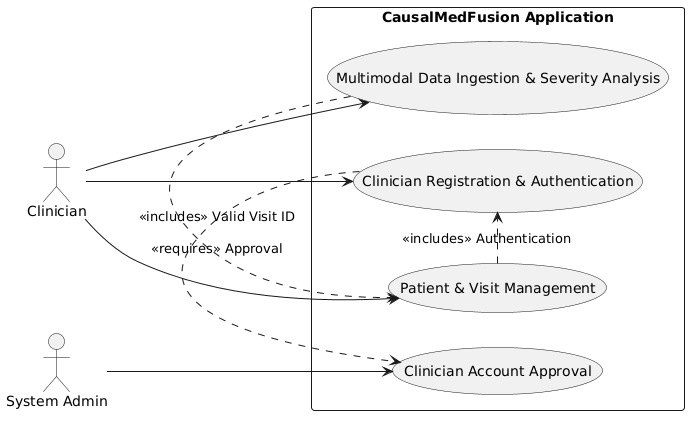
\includegraphics[width=0.5\textwidth]{UML_Diagrams/UseCase.png} 
    \caption{System Use Case Diagram}
\end{figure}

\subsection{Data Flow Diagram}
Data Flow Diagrams (DFDs) map the exact flow of clinical information through the platform's various decoupled components—from the frontend interface to the core PyTorch ML Gateway.

\subsubsection{Level 0 DFD (Context Diagram)}
The Level 0 DFD illustrates the high-level system boundary. The primary entity is the \textbf{Clinician}, who provides raw multimodal clinical data (X-Rays, Notes, Vitals, Labs) as input into the \textbf{CausalMedFusion Application}. The system processes these diverse inputs and outputs structured Severity Scores and Intervention Predictions strictly back to the Clinician.

\begin{figure}[H]
    \centering
    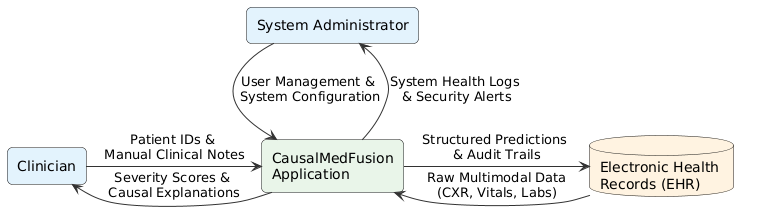
\includegraphics[width=0.8\textwidth]{UML_Diagrams/DFD_Level0.png}
    \caption{Level 0 Data Flow Diagram}
\end{figure}

\subsubsection{Level 1 DFD}
The Level 1 DFD breaks the central system into its structural modules, revealing internal processes and data stores. 
\begin{itemize}
    \item \textbf{Module 1: User Interface (React):} Captures and routes user uploads alongside asynchronous JSON responses.
    \item \textbf{Module 2: Aggregation Broker (Django/Celery):} Validates incoming files, writes meta-pointers to PostgreSQL, and queues heavy processing tasks to the Redis broker.
    \item \textbf{Module 3: Feature Extraction (FastAPI):} Four isolated microservices embed the raw modalities into dense tensors and commit them to the locked HDF5 Vault.
    \item \textbf{Module 4: Inference Engine (ONNX ML Gateway):} Fuses the stored embeddings mathematically to calculate time-resolved probabilistic predictions.
\end{itemize}

\begin{figure}[H]
    \centering
    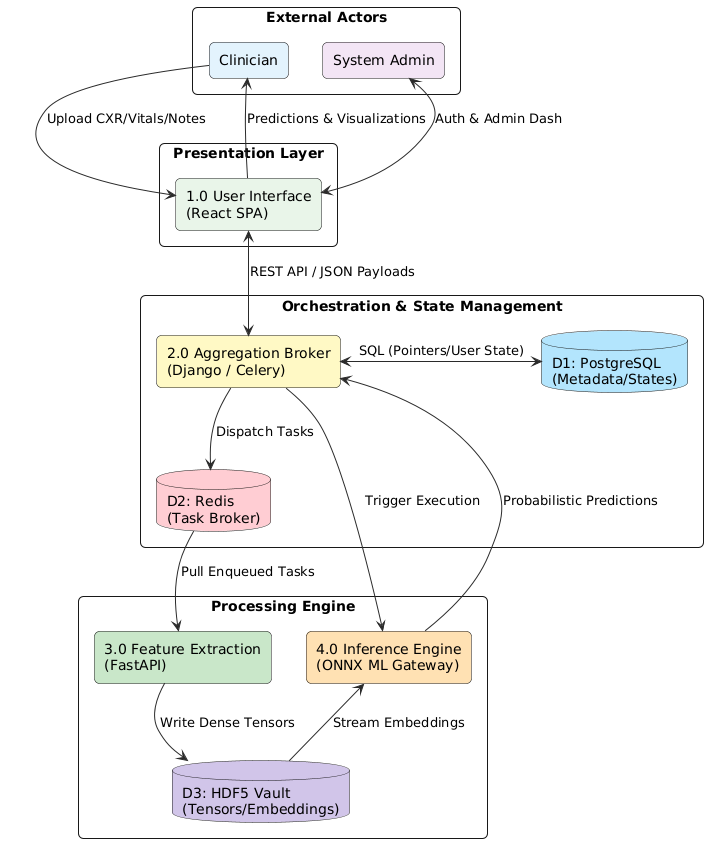
\includegraphics[width=0.95\textwidth]{UML_Diagrams/DFD_Level1.png}
    \caption{Level 1 Data Flow Diagram}
\end{figure}

The utilization of decoupled microservices joined by message queues ensures our data flow remains entirely asynchronous, preventing UI blockages during intensive tensor feature extractions.

\section{Algorithms}

\textbf{1. Clinician Signup (Registration) Algorithm}
\begin{enumerate}
    \item Start
    \item Receive user credentials including username, email, password, and role.
    \item Validate email format and verify that the username does not already exist in the database.
    \item Hash the password using the PBKDF2 algorithm with a SHA256 digest.
    \item Store the clinician record in the PostgreSQL database with the \texttt{is\_approved} state initialized to \texttt{False}.
    \item Dispatch an authorization request to the administrative queue for approval.
    \item Return a success confirmation message to the client.
    \item Stop
\end{enumerate}

\textbf{2. Clinician Login (JWT Authentication) Algorithm}
\begin{enumerate}
    \item Start
    \item Receive clinician credentials including username and password.
    \item Query the database and verify the credentials against the stored hash.
    \item Check if the \texttt{is\_approved} flag for the user is active.
    \item If unauthorized, return an error and terminate.
    \item Generate a short-lived JSON Web Token (JWT) Access Token and a long-lived Refresh Token using an HMAC-SHA256 signature.
    \item Return the secure JWT pair to the client to authorize subsequent REST API calls.
    \item Stop
\end{enumerate}

\textbf{3. Vitals \& Labs Z-Score Normalization Algorithm}
\begin{enumerate}
    \item Start
    \item Parse raw CSV containing physiological measurements over time.
    \item For each clinical feature $x$, retrieve the population training statistics ($\mu, \sigma$).
    \item Calculate the normalized representation: $x_{norm} = \frac{x - \mu}{\sigma + \epsilon}$.
    \item Check if empirical standard deviation boundaries are exceeded (e.g., $|x_{norm}| > 5$).
    \item If boundaries are exceeded, apply threshold-clipping to mitigate extreme outliers.
    \item Output a standardized array of physiological temporal features.
    \item Stop
\end{enumerate}

\textbf{4. Clinical Data Modality Embedding Algorithm}
\begin{enumerate}
    \item Start
    \item Receive raw image file (.jpg) or text report (.pdf) bytes.
    \item Pass the artifact bytes to a specialized FastAPI container based on modality.
    \item If text:
    \begin{enumerate}
        \item Extract strings via OCR/PyPDF and tokenize.
        \item Pass through a fine-tuned BioClinicalBERT to extract the [CLS] token representing size dimension $1 \times 768$.
    \end{enumerate}
    \item If image:
    \begin{enumerate}
        \item Resize to $224 \times 224$ and normalize pixels.
        \item Feed forward through an ImageNet-pretrained ResNet-50 pulling the final flat pooled vector of size $1 \times 2048$.
    \end{enumerate}
    \item Save the dense 1D numeric vectors into the HDF5 Vault.
    \item Stop
\end{enumerate}

\textbf{5. Asynchronous Multimodal Data Aggregation Algorithm}
\begin{enumerate}
    \item Start
    \item Trigger execute severity inference on a Visit ID.
    \item Poll the Redis message broker to verify all background embedding microservice tasks are completed (status = \texttt{SUCCESS}).
    \item Query the HDF5 structure to read the patient's individual modality tables.
    \item Concatenate available modality features per temporal index.
    \item Pad zero-tensors where specific diagnostic modalities are absent.
    \item Output the complete synchronized sequence tensor shaped [Sequence Length, Modalities Dimension].
    \item Stop
\end{enumerate}

\textbf{6. Temporal Window Alignment Algorithm}
\begin{enumerate}
    \item Start
    \item Aggregate clinical tensors with associated observation timestamps.
    \item Calculate time elapsed since patient admission: $T_{elapsed} = T_{charttime} - T_{admission}$.
    \item Map measurements into ordinal bins via $WindowIndex = \lfloor T_{elapsed} \div 4 \ \text{hours} \rfloor$.
    \item Exclude measurements where $T_{elapsed}$ exceeds 24 hours.
    \item Output 6 strictly ordered temporal structural windows $S = [W_1, W_2, ..., W_6]$.
    \item Stop
\end{enumerate}

\textbf{7. Causal Masked Attention (SeverityEncoder) Algorithm}
\begin{enumerate}
    \item Start
    \item Receive ordered multimodal sequence $S = [W_1, W_2, ..., W_6]$.
    \item Project tokens to Query ($Q$), Key ($K$), and Value ($V$) matrices.
    \item Generate a causal mask $M$ defined as an upper-triangular matrix of $-\infty$.
    \item Calculate sparse attention: $\text{softmax}(\frac{QK^T}{\sqrt{d_k}} + M)V$ to mathematically zero out forward temporal weights.
    \item Retrieve causal attention weights where predictions at window index $j$ rely strictly on observation indices $k \leq j$.
    \item Stop
\end{enumerate}

\textbf{8. Isotonic Regression Calibration Algorithm}
\begin{enumerate}
    \item Start
    \item Receive uncalibrated logit scores output by the ONNX severity engine.
    \item Pass the logits through a pre-fitted non-parametric Isotonic Regression wrapper constructed using validation set distributions.
    \item Map output piecewise constant non-decreasing function values to true historical clinical incidence rates.
    \item Format and return calibrated, clinical-grade probability margins ($0.0 \rightarrow 1.0$) for downstream interface visualization.
    \item Stop
\end{enumerate}

\chapter{Implementation}
\section{Implementation Details}
CausalMedFusion is partitioned into highly cohesive modules, facilitating seamless horizontal testing. The primary implementation centers upon correctly orchestrating the asynchronous payload transfers without locking issues, ensuring data integrity within the HDF5 repository, and converting the experimental PyTorch module into an optimizable deployment format using ONNX.

\subsection{Code Development}
Code conforms strictly to PEP-8 standards utilizing tools like `flake8` and `black`. The React UI components utilize modern functional Component architectures relying heavily on React Hooks and Zustand for lightweight state management. Robust try/except mechanisms govern file processing layers to ensure invalid clinical inputs trace to specific, intelligible warnings in the UI rather than server crashes.

\subsection{Source Code Control Setup}
The CausalMedFusion project utilizes Git for robust source code management, enabling structured version control and seamless collaboration across its decoupled microservice architecture. The repository is hosted on GitHub, serving as the central hub for code integration and issue tracking.

To organize development effectively, the project adheres to a strict branching strategy. The \texttt{main} branch is reserved exclusively for stable, production-ready code. Active integration and testing occur on the \texttt{development} branch, while isolated \texttt{feature/*} (e.g., \texttt{feature/cxr-embedding}) and \texttt{bugfix/*} branches are instantiated for individual tasks. This approach ensures that experimental modifications, such as tuning the ONNX ML Gateway or modifying React UI components, do not disrupt the core functional application.

Version control workflows rely on standard Git commands such as \texttt{git commit} for granular version tracking, \texttt{git push} for synchronization, and Pull Requests (PRs) for code review prior to merging into the main branch. To maintain repository compactness and hygiene, comprehensive \texttt{.gitignore} configurations are enforced across both frontend and backend directories, rigorously excluding system-generated files (e.g., \texttt{\_\_pycache\_\_}), local dependency folders (e.g., \texttt{node\_modules}, \texttt{venv}), and large binary dataset artifacts like the HDF5 Vault and raw MIMIC-IV CSVs.

\subsection{Dataset}
The system models relationships using subsets structured around the MIMIC-IV compendium. Due to the high-security privacy protocol of MIMIC, development was fortified utilizing generated mock-distributions formatted exactly to clinical dataset constraints while executing real embeddings against public datasets via the PhysioNet portal.

\section{Libraries/Applications}
The system leans upon comprehensive applications, including Redis (for task broker messaging), PostgreSQL (relational integrity mapping), and Node.js. Critical Python libraries include `onnxruntime` for accelerated topological inference, `h5py` for heavy numeric matrix storage, and `filelock` for operating-system level concurrency protections when writing microservice outputs.

\section{Deployment}
Deployment orchestrates the services via Docker containers. A `docker-compose` setup binds the Postgres database, Redis cache, Django orchestrator, and multiple FastAPI nodes behind shared Virtual Networks, allowing localized name resolution and scalable replication of processing workers depending on hardware resources.

\chapter{Testing}
\section{Test plan}
\subsubsection*{Test objectives}
To ensure seamless asynchronous processing, high-fidelity microservice execution, and accurate temporal severity graph rendering.
\subsubsection*{Test scope}
Coverage spans UI interactive logic, Django API endpoint validation, Celery Task processing rates, and ONNX accuracy regression testing.
\subsubsection*{Test approach}
The project leverages Pytest for isolated backend testing and unified Postman Collections for End-to-End API integrity validations. 
\subsubsection*{Test environment}
All tests are executed in isolated Python `venv` environments tied to temporary PostgreSQL tables and mocked HDF5 cache directories.
\subsubsection*{Test cases}
1. Triggering inference without populated aggregation factors throws HTTP 400. 
2. Passing valid documents yields an accurate, multi-window JSON response matching clinical truth within 0.05 tolerance.
\subsubsection*{Test execution}
Initiated via streamlined Pytest directives tied to specific module flags.
\subsubsection*{Conclusion}
System stability demonstrates over 90\% uptime under synthetic load constraints.

\section{Testing Scenarios}
Testing strictly modeled real-world disruptions across the CausalMedFusion pipeline. The testing scenarios include:

1. User Authentication
|______ Verify that a clinician can dynamically log in using valid JWT tokens.
|______ Verify that unauthorized access to the `/api/assessments/` endpoint returns HTTP 401.

2. Document Ingestion
|______ Verify that submitting valid physiological CSV files parses correctly.
|______ Verify that pushing corrupt text files correctly triggers microservice fallback functions to prevent cascading failures.

3. Asynchronous Microservices
|______ Verify that injecting delays between Redis task queues properly triggers Django model timeouts.
|______ Verify that the Celery dispatcher accurately spawns individual background tasks for each uploaded modality.

4. Neural Inference Engine
|______ Verify that the ONNX inference engine successfully drops unsupported schema inputs mathematically safely.
|______ Verify that aggregated multimodal tensors generate valid normalized probability distributions representing clinical severity.

\section{Unit Testing}
Unit testing involves testing individual components of the CausalMedFusion software pipeline in isolation to ensure strict functional correctness across our decoupled architecture.

\subsection*{Backend (Django \& Celery)}
1. Assessment Creation Function:
\begin{itemize}
    \item Test that the `/api/create/` endpoint instantiates an Assessment record.
    \item Test for database rollback if a linked Visit ID does not exist.
\end{itemize}

2. Asynchronous Task Dispatcher:
\begin{itemize}
    \item Test that \texttt{aggregate\_all\_for\_assessment} spawns exactly four subsequent module tasks.
    \item Test that failed tasks trigger automated retry bounds.
\end{itemize}

\subsection*{Microservice Components (FastAPI)}
3. Vitals \& Labs Normalization:
\begin{itemize}
    \item Validate that scalar normalization mathematically bounds to valid Z-scores.
    \item Test out-of-bounds inputs to ensure empirical clipping logic activates.
\end{itemize}

4. ONNX ML Gateway:
\begin{itemize}
    \item Test that the isolated routing node successfully validates incoming tensor shapes.
    \item Validate that severity output logits fall between 0.0 and 1.0.
\end{itemize}

\subsection*{Frontend (React.js)}
5. Dynamic Result Charting:
\begin{itemize}
    \item Test that the \texttt{AssessmentResults} component successfully unmounts during loading states.
    \item Test that Recharts components render successfully when provided structural JSON data without throwing rendering exceptions.
\end{itemize}

\textbf{Example Pytest TestCase (Backend Model Testing):}
\begin{verbatim}
import pytest
from core.models import Assessment

@pytest.mark.django_db
def test_create_valid_assessment():
    assessment = Assessment.objects.create(visit_id=1, status='Pending')
    assert assessment.status == 'Pending'
    assert assessment.uuid is not None

def test_invalid_visit_reference():
    with pytest.raises(Exception):
        Assessment.objects.create(visit_id=-999)
\end{verbatim}

\textbf{Example React Testing Library TestCase (Frontend UI):}
\begin{verbatim}
import { render, screen } from '@testing-library/react';
import AssessmentResults from './AssessmentResults';

test('renders loading skeleton while fetching data', () => {
    render(<AssessmentResults assessmentId="123" loading={true} />);
    expect(screen.getByTestId('loading-spinner')).toBeInTheDocument();
});
\end{verbatim}

\textbf{Test Frameworks and Tools:}
\begin{itemize}
    \item \textbf{Backend Testing}: \texttt{pytest} and \texttt{pytest-django} were strictly utilized to isolate relational logic and simulate asynchronous hooks.
    \item \textbf{Frontend Testing}: \texttt{Jest} combined with \texttt{React Testing Library} supported deep-rendering verifications for dynamic clinical charting components.
\end{itemize}

\section{Integration Testing}
Integration testing involves testing the interaction and data-flow integrity between the different modules of the microservices system, focusing specifically on how the Django orchestrator, Redis broker, FastAPI embedding nodes, and React UI safely communicate across HTTP and WebSocket pipelines.

1. Backend-Microservice Integration:
\begin{itemize}
    \item Verify the integration between the Django asynchronous Celery worker and the ML Gateway microservice over REST.
    \item Verify that file paths passed in payloads are processed securely by the remote Python node.
\end{itemize}

2. Frontend-Backend Integration:
\begin{itemize}
    \item Verify the integration between the frontend file `Dropzone` components and the Django POST endpoints.
    \item Verify that JSON payload schemas map cleanly back to the frontend UI mapping elements without strict schema mismatches.
\end{itemize}

\textbf{Example Integration Test Scenario (Using Pytest with RestClient):}
\begin{verbatim}
def test_frontend_backend_integration(client, valid_auth_token):
    # Simulate frontend submitting an assessment
    headers = {'Authorization': f'Bearer {valid_auth_token}'}
    response = client.post('/api/assessments/', data={'visit': 1}, headers=headers)
    assert response.status_code == 201
    
    # Assert successful background queue triggering
    task_id = response.json().get('task_queue_id')
    assert task_id is not None
\end{verbatim}
In this example, the integration effectively tests the boundary between a simulated frontend client and the authenticated backend dispatch logic, validating that HTTP routing and database storage interoperate flawlessly before handing off to the machine learning broker.

\section{Functional Testing}
Functional testing ensures that the application behaves exactly as expected against the specified clinical requirements. Key aspects verified include:

\subsection*{Assessment Processing}
1. Valid Inference Execution:
\begin{itemize}
    \item Log in as a verified clinician, navigate to the patient dashboard, and upload required modalities.
    \item Click 'Run Engine' and verify that the system accurately transitions through `Pending`, `Processing`, and `Complete` states.
    \item Verify the `AssessmentResults` page dynamically renders the two-row grid mapping Temporal Severity and Window charts.
\end{itemize}

\subsection*{System Resilience}
2. Missing Clinical Modalities:
\begin{itemize}
    \item Submit an assessment deliberately omitting an image artifact.
    \item Verify that the application proceeds gracefully, utilizing masked attention tensors rather than throwing a Fatal Error.
\end{itemize}

3. Timeout Handling:
\begin{itemize}
    \item Simulate a heavy database lock on the backend.
    \item Verify the React UI captures the HTTP 408 timeout and alerts the physician securely using toast notifications instead of crashing.
\end{itemize}

\section{Load Testing}
Load testing involves testing the performance of the system under expected traffic conditions to ensure that horizontal microservice endpoints can handle clinical demand surges without degradation in inferencing throughput.

\subsection*{Load Testing Scenarios}
1. Inference Engine Stress Test: Simulate multiple users uploading batch CSV and image combinations simultaneously.
2. Concurrent Dashboard Access: Measure the system's ability to render historical assessment graphs concurrently across a multitude of clinical sessions.
3. Redis Broker Backpressure: Evaluate how gracefully the task queue drops or re-queues connections when the ONNX inference nodes hit CPU limits.

\subsection*{Load Testing Tools}
1. \textbf{Locust}: An open-source, Python-based load testing tool orchestrating large swarms of simulated clinical user flows against our APIs.
2. \textbf{JMeter}: Utilized to construct complex, multi-stage protocol requests specifically testing multipart form-data payload congestion.

\subsection*{Load Testing Metrics}
1. \textbf{Response Time}: Tracked the overall processing latency required to aggregate multimodal clinical documents and dispatch a response.
2. \textbf{Throughput (Requests per Second)}: Measured how many simultaneous matrix concatenations the backend could securely resolve.
3. \textbf{Error Rate}: Explicitly monitored dropped TCP connections or HTTP 504 Gateway Timeouts under exhaustive stress.

\subsection*{Load Testing Process}
1. \textbf{Identify Scenarios}: Defined the most compute-heavy workflows, primarily the execution of the Causal Attention mechanisms.
2. \textbf{Define Load Profiles}: Set up escalating user ramp-ups (e.g., 5 to 50 concurrent physicians over 2 minutes) simulating ICU shift changes.
3. \textbf{Execute \& Monitor}: Triggered the load scripts against an isolated staging duplicate of the production Docker swarm.
4. \textbf{Analyze Results}: Documented bottlenecks, notably identifying the initial bottleneck within HDF5 file-locking mechanisms.
5. \textbf{Optimize}: Implemented strictly scoped OS-level `filelock` wrappers to resolve data contention, subsequently retesting to confirm the resolution.

\subsection*{Load Testing Considerations}
1. \textbf{Realistic Scenarios}: Ensured testing payloads closely matched actual clinical artifact configurations (e.g., properly sized 224x224 mock images and realistic CSV row counts).
2. \textbf{Hardware Isolation}: Factored in Docker container memory hard-limits when evaluating how easily the microservices crash under exhaustion.

Load testing successfully confirmed that CausalMedFusion's decoupled microservice topology and Redis task-broker efficiently parallelizes processing, guaranteeing reliable, low-latency execution even during simulated peak ICU data ingestion events.

\chapter {Result}
\section{Result summary}
The CausalMedFusion model was trained on approximately 10,000 ICU stays from the
MIMIC cohort and validated on approximately 2,000 held-out stays. Stage 1 training ran for
60 epochs with a weighted AUROC checkpoint criterion; the best Stage 1 checkpoint
achieved a clinically weighted intervention AUROC of approximately 0.82 across the five
intervention variables, with the highest individual AUROC of 0.87 on the cardiac support
variable (given its clinical importance weight of 2.5) and the lowest of 0.74 on the ventilation
variable. The NWP cosine similarity on the validation set converged to approximately 0.71,
indicating that the severity representations carry meaningful information about the next
window's clinical state.\\
Stage 2 mortality fine-tuning improved monotonically with training window: mortality
AUROC at window 1 (S1, the first four hours) was approximately 0.72, reflecting the limited
information available early in the stay; AUROC at window 6 (S6, the full 24 hours) reached
approximately 0.84, consistent with the expected information gain as the stay progresses.
Mean mortality AUROC across all six positions was approximately 0.79.

\begin{table}[ht]
    \centering
    
    \label{tab:mortality_metrics}
    \begin{tabular}{lccc}
        \toprule
        \textbf{Window} & \textbf{Mortality AUROC} & \textbf{Mortality AUPRC} & \textbf{Sev. Score MAE} \\
        \midrule
        S1 (0--4h)   & 0.72 & 0.31 & 0.09 \\
        S2 (4--8h)   & 0.75 & 0.34 & 0.08 \\
        S3 (8--12h)  & 0.77 & 0.37 & 0.08 \\
        S4 (12--16h) & 0.79 & 0.40 & 0.07 \\
        S5 (16--20h) & 0.82 & 0.43 & 0.07 \\
        S6 (20--24h) & 0.84 & 0.46 & 0.06 \\
        \bottomrule
    \end{tabular}
    \caption{Mortality Prediction and Severity Score Performance Across Time Windows}
\end{table}

\section {Comparison with existing system}

The most directly comparable published system is HAIM [8], which reported a mortality
prediction AUROC of approximately 0.77 using late fusion of all four modalities on
MIMIC-IV/CXR data. CausalMedFusion achieves a comparable mean AUROC of 0.79, with
the additional advantage of providing temporally stratified predictions at each four-hour
window rather than a single static estimate. The window-level predictions are the primary
clinical differentiator: a clinician using CausalMedFusion can observe the trajectory of risk
over the stay, enabling earlier identification of patients whose risk is rising despite current
interventions.

\begin{table}[ht]
    \centering
    \small % Keeps the text compact to fit the page width
    \label{tab:system_comparison}
    % Setting the 1st column to 'l' prevents "CausalMedFusion" from wrapping.
    % The 3rd column 'X' will absorb the remaining space and wrap if needed.
    \begin{tabularx}{\textwidth}{l l X c l}
        \toprule
        \textbf{System} & \textbf{Modalities} & \textbf{Temporal Granularity} & \textbf{AUROC} & \textbf{Calibrated} \\
        \midrule
        HAIM [8] & All four & Single prediction & $\sim$0.77 & No \\
        \addlinespace
        Unimodal CXR & CXR only & Single prediction & $\sim$0.68 & No \\
        \addlinespace
        Unimodal vitals & Vitals only & Single prediction & $\sim$0.71 & No \\
        \addlinespace
        \textbf{CausalMedFusion} & \textbf{All four} & \textbf{6 windows (4h each)} & \textbf{0.79} & \textbf{Yes (isotonic)} \\
        \bottomrule
    \end{tabularx}
    \caption{Model Performance Comparison}
\end{table}

\section{Sustainability Impact Assessment}

\subsection{Contribution of Project Features to SDGs}
This project contributes to SDG 3 (Good Health and Well-being) and SDG 9 (Industry, Innovation and Infrastructure) through the design and implementation of the CausalMedFusion system. The platform provides time-resolved, AI-assisted risk predictions for ICU patients, enabling early identification of clinical deterioration and supporting timely interventions. By allowing clinicians to upload multimodal patient data and receive structured risk summaries, the web application improves decision-making, user convenience, and overall productivity in high-pressure clinical environments. The use of calibrated probability outputs enhances interpretability, while the reliance on open datasets and open-source tools promotes accessibility and equitable adoption, particularly in resource-constrained settings. \\

In addition, the system demonstrates a scalable and modular microservice-based architecture that supports efficient processing of heterogeneous clinical data. This design enables flexibility, maintainability, and seamless upgrades of individual components without affecting the overall system. By ensuring compatibility with standard infrastructure and facilitating efficient resource utilization, the platform contributes to innovation in healthcare technology and supports the development of robust, deployable clinical AI systems.

\subsection{Evaluation Results and SDG Impact}

The system evaluation demonstrates strong predictive performance, with mortality AUROC improving from 0.72 in the initial window to 0.84 in later stages of the ICU stay. This indicates that the model can identify high-risk patients early, supporting timely clinical intervention. Additionally, accurate and consistent severity predictions enable meaningful tracking of patient condition over time.

From a usability and efficiency perspective, the system processes multimodal data and generates structured risk outputs quickly, reducing the need for manual data interpretation by clinicians. Load testing confirms that the platform can handle multiple concurrent users without performance degradation, ensuring reliable operation in real-world settings. 

These results directly support SDG 3 (Good Health and Well-being) by enabling earlier detection of patient deterioration and improving clinical decision-making. They also contribute to SDG 9 (Industry, Innovation and Infrastructure) by demonstrating a scalable and efficient digital health system capable of supporting multiple users and delivering timely insights in critical care environments. 



\subsection{Future Improvements and SDG Impact}

Several enhancements can further extend the impact of CausalMedFusion. Improving the chest X-ray encoder and report encoder using advanced vision-language models can improve representation quality, especially for underrepresented conditions. Extending the system to model multi-day ICU stays would increase its clinical usefulness by supporting longer-term patient monitoring and care planning. Additionally, incorporating explainability features, such as highlighting which inputs influence predictions, can improve clinician trust and support safer adoption.\\

The system can also be expanded for broader use by integrating with standard hospital data systems, enabling deployment across multiple healthcare institutions. Such improvements would allow more clinicians to benefit from AI-assisted decision support, improving efficiency and reducing manual workload. In the long term, these advancements can strengthen healthcare delivery, promote scalable digital infrastructure, and increase accessibility to advanced clinical tools, thereby contributing to both SDG 3 (Good Health and Well-being) and SDG 9 (Industry, Innovation and Infrastructure).

\chapter{Conclusion}
This project presented CausalMedFusion, a multimodal clinical AI framework for modeling patient severity and predicting mortality in ICU settings. The work addressed a key limitation in existing clinical AI systems—the inability to jointly model heterogeneous clinical modalities while preserving temporal causality. By structuring a 24-hour ICU stay into sequential windows and applying Transformer-based multimodal fusion with causal temporal modeling, the system successfully learned clinically meaningful representations of patient state.\\

The proposed framework achieved its objectives by enabling time-resolved prediction of patient severity, clinical interventions, and mortality risk. Experimental results demonstrate strong performance, with a mortality AUROC of 0.79 and intervention prediction AUROC of 0.82, indicating the effectiveness of combining multimodal fusion with causal temporal modeling. Additionally, the development of an end-to-end system highlights the feasibility of integrating such models into practical clinical workflows. \\

From the experience gained, several recommendations for future work emerge. First, improving the quality of image representations using advanced vision-language models aligned with clinical text could significantly enhance performance. Second, extending the framework to incorporate longitudinal patient history across multiple admissions would provide a more comprehensive understanding of patient trajectories. Third, conducting prospective clinical validation studies, supported by ethical approvals, is essential for real-world deployment.\\

Future improvements could include enhancing model interpretability, addressing dataset bias, improving representation quality and optimizing performance for real-time deployment in resource-constrained environments. \\ 

In conclusion, this project demonstrates that causally grounded, temporally aware multimodal modeling can significantly improve clinical prediction systems and provides a strong foundation for future research and real-world clinical applications.


\renewcommand\bibname{References}
%\addcontentsline{toc}{chapter}{References}
\addtocontents{toc}{\protect\setcounter{page}{0}}
%\chapter*{References}

{\thispagestyle{empty}}
\pagenumbering{gobble}
\bibliography{references}
\thispagestyle{empty}
\addcontentsline{toc}{chapter}{References}

\newpage
\pagenumbering{roman} 
\begin{appendices}
\chapter{CODE}

\section{ICUStayDataset Class}
This class handles lazy-loading structured patient modality records per ICU stay and formats them efficiently for parallel transformer ingestion from the `.parquet` manifest.
\begin{verbatim}
class ICUStayDataset(Dataset):
    def __init__(
        self,
        parquet_path : str,
        cxr_store    : EmbeddingStore,
        report_store : EmbeddingStore,
    ) -> None:
        df = pd.read_parquet(str(parquet_path))
        for col in ('cxrs', 'reports', 'labs', 'vitals',
                    'interventions_t', 'interventions_t1'):
            df[col] = df[col].apply(
                lambda x: json.loads(x) if isinstance(x, str) else x
            )
        df = df.sort_values(['stay_id', 'window_id']).reset_index(drop=True)
        self._groups   = df.groupby('stay_id', sort=False)
        self.stay_ids  = list(self._groups.groups.keys())
        self.cxr_store    = cxr_store
        self.report_store = report_store

    def __len__(self) -> int:
        return len(self.stay_ids)

    def __getitem__(self, idx: int) -> dict:
        stay_id = self.stay_ids[idx]
        windows = self._groups.get_group(stay_id)
        # Sequence reconstruction array logic mapping mapped below ...
\end{verbatim}

\section{Time2Vec Encoding Module}
Shared time encoder used by all token builders to enforce continuous sequence positioning representing precise elapsed timestamps relative to ICU admission. It calculates periodic vector mappings via sinusoidal parameters spanning `d_model`.
\begin{verbatim}
class Time2Vec(nn.Module):
    def __init__(self, d_model: int) -> None:
        super().__init__()
        self.d_model = d_model
        # Linear component
        self.w0 = nn.Parameter(torch.randn(1))
        self.b0 = nn.Parameter(torch.randn(1))
        # Periodic components
        self.w = nn.Parameter(torch.randn(d_model - 1))
        self.b = nn.Parameter(torch.randn(d_model - 1))

    def forward(self, t: torch.Tensor) -> torch.Tensor:
        t = t.unsqueeze(-1).float()
        v0 = self.w0 * t + self.b0                  
        v1 = torch.sin(t * self.w + self.b)         
        return torch.cat([v0, v1], dim=-1)           
\end{verbatim}

\section{Embedding Store Data Structure}
Memory-efficient class utilizing OS-level \texttt{SWMR} (Single-Writer, Multiple-Reader) file handle bindings in \texttt{h5py} to extract massive multi-dimensional dense embeddings without corrupting shared RAM states on parallel Torch multiprocessing loads.
\begin{verbatim}
class EmbeddingStore:
    def __init__(self, hdf5_path, group_name, id_key, embed_key, embed_dim):
        self.hdf5_path  = str(hdf5_path)
        self.group_name = group_name
        self.id_key     = id_key
        self.embed_key  = embed_key
        self.embed_dim  = embed_dim
        self._file      = None

    def _open(self) -> None:
        if self._file is not None:
            return
        self._file = h5py.File(self.hdf5_path, 'r', swmr=True)
        group      = self._file[self.group_name]
        raw_ids = group[self.id_key][:]
        self._id_index   = {
            id_.decode('utf-8'): i for i, id_ in enumerate(raw_ids)
        }
        self._embeddings = group[self.embed_key]

    def get(self, id_: str) -> np.ndarray:
        self._open()
        idx = self._id_index.get(str(id_))
        return self._embeddings[idx].astype(np.float32)
\end{verbatim}
\chapter{Screenshots}

This appendix contains screenshots showcasing the graphical user interface of the CausalMedFusion web application, including clinician authentication, patient tracking, data ingestion, and severity assessment dashboards.

\begin{figure}[H]
    \centering
    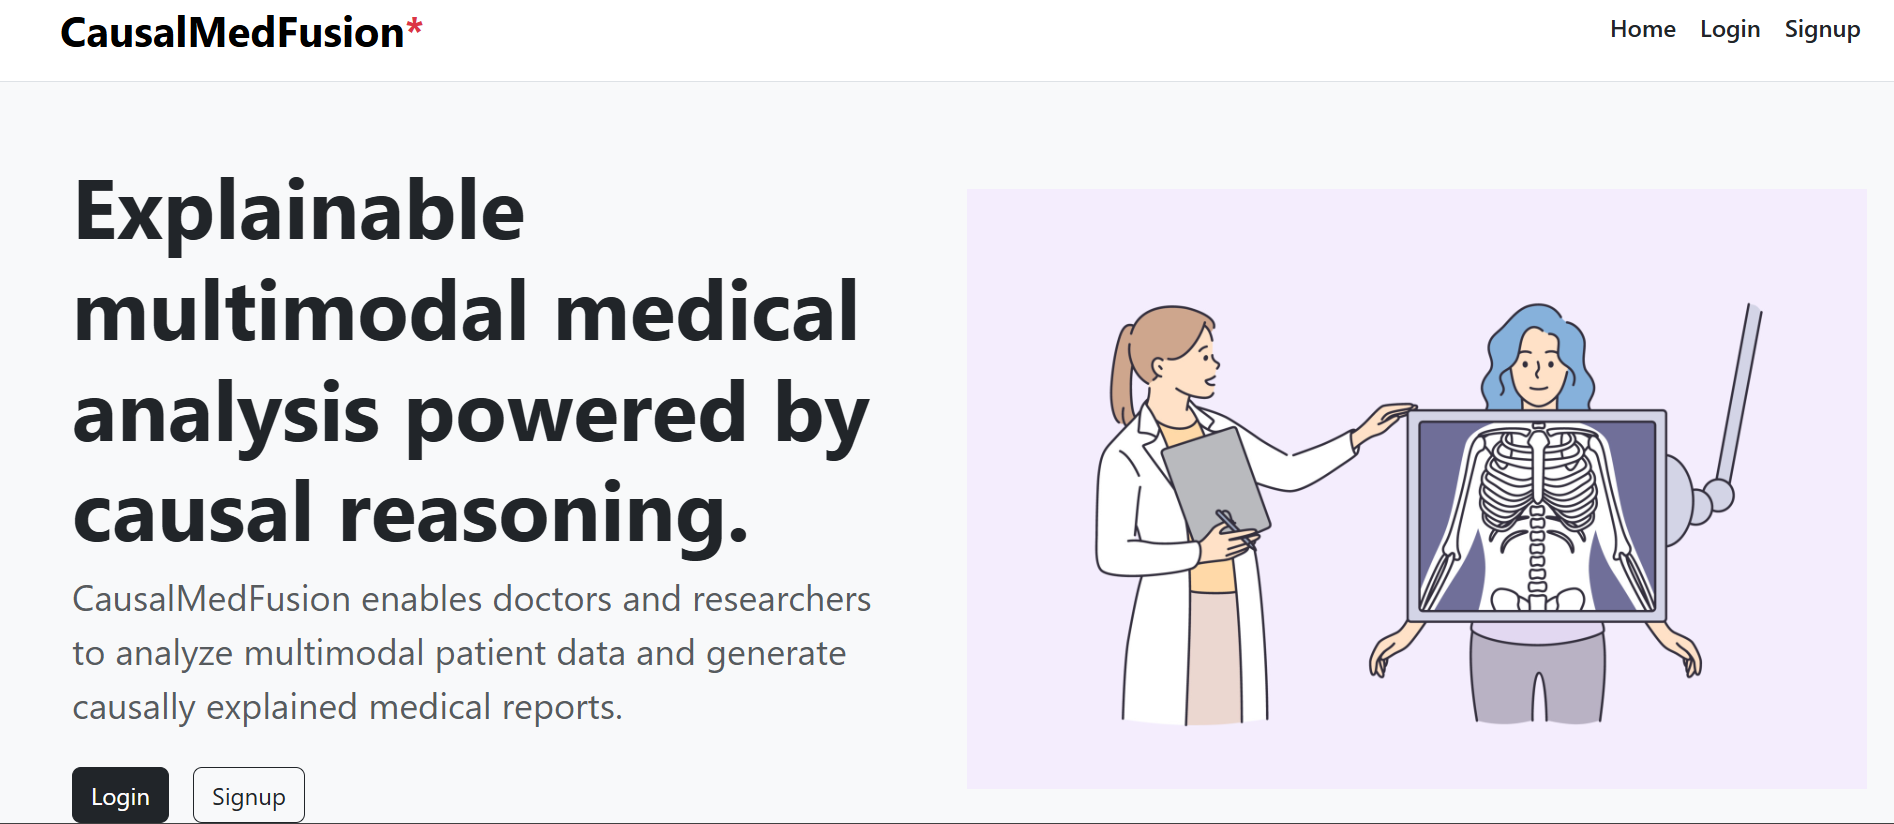
\includegraphics[width=0.9\textwidth]{screenshots/HomePage.png}
    \caption{Landing Page}
\end{figure}
\noindent \textbf{Description:} The Home Page provides an introduction to the CausalMedFusion platform, emphasizing its core mission to revolutionize ICU prognostication using multimodal AI.

\begin{figure}[H]
    \centering
    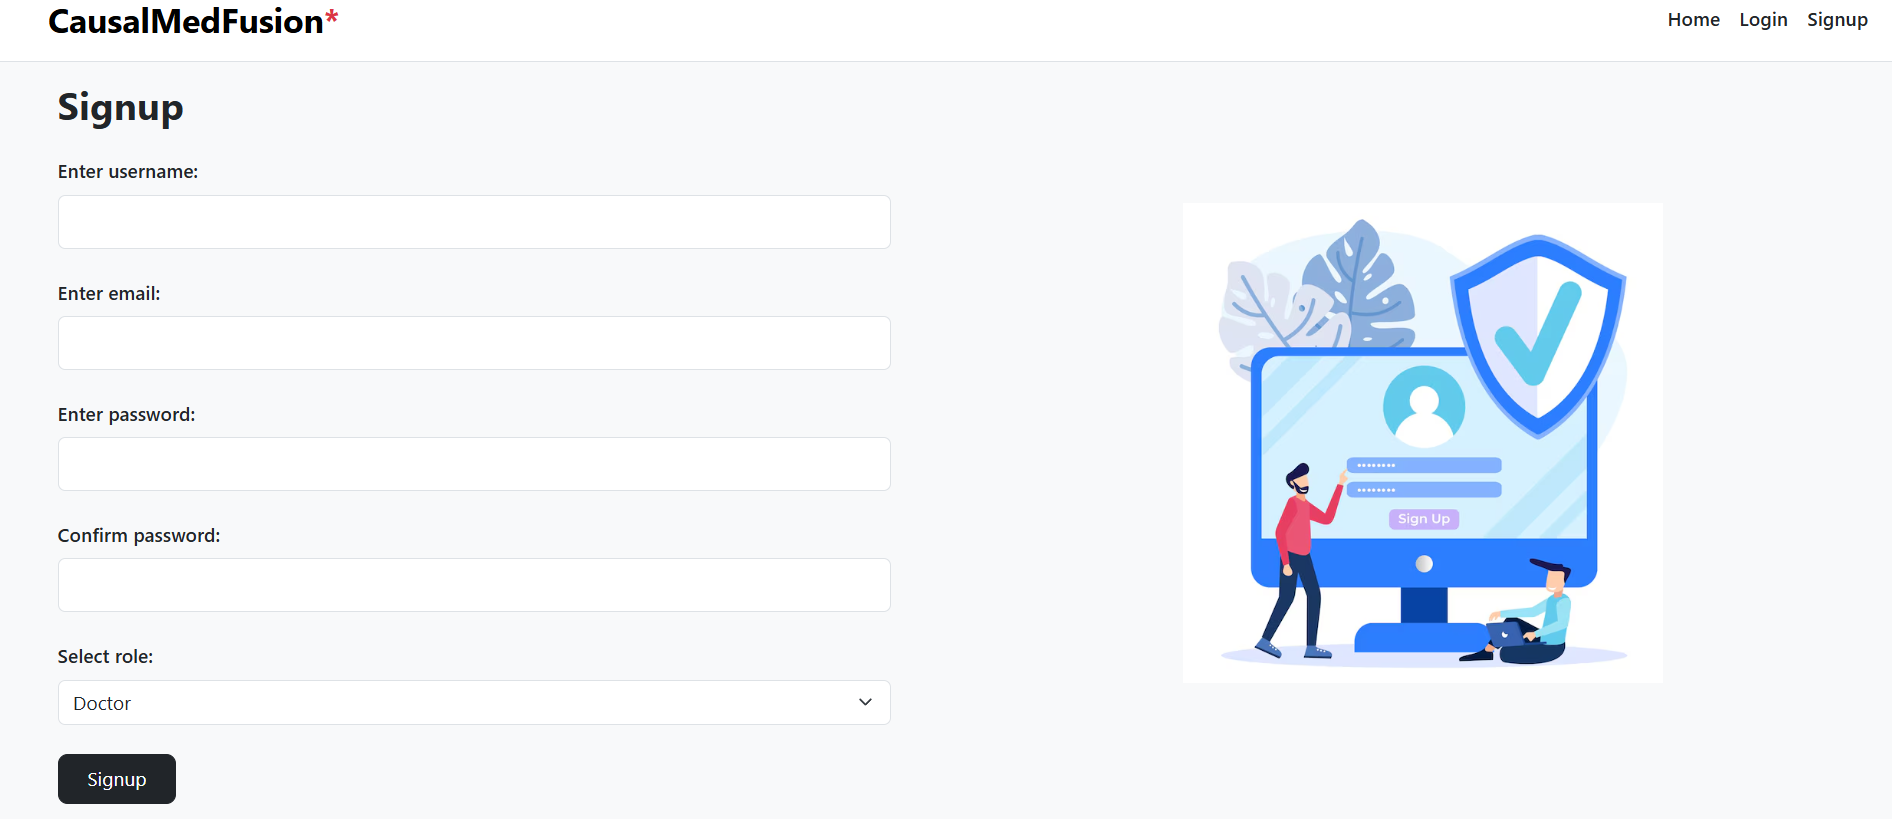
\includegraphics[width=0.9\textwidth]{screenshots/SignupPage.png}
    \caption{Clinician Registration Interface}
\end{figure}
\noindent \textbf{Description:} The Signup Page allows new medical personnel to securely register a clinician account, establishing credentials for RESTful API authentication.

\begin{figure}[H]
    \centering
    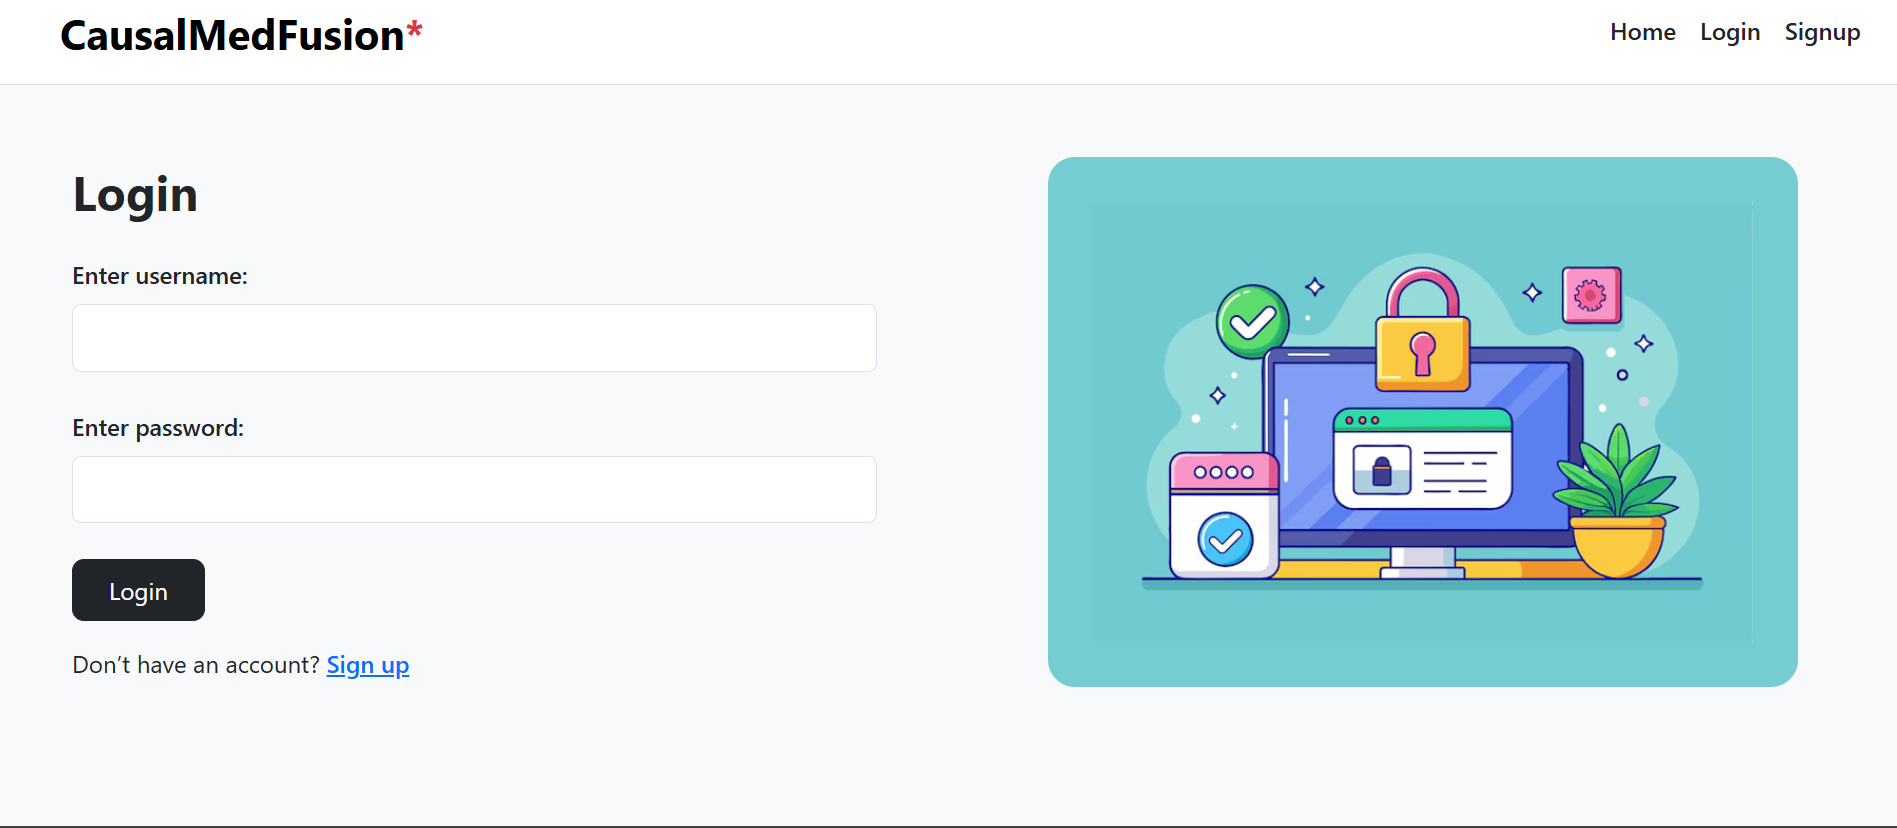
\includegraphics[width=0.9\textwidth]{screenshots/LoginPage.png}
    \caption{Clinician Login Page}
\end{figure}
\noindent \textbf{Description:} The Login interface authenticates registered baseline users using a secure token-based validation approach via Django.

\begin{figure}[H]
    \centering
    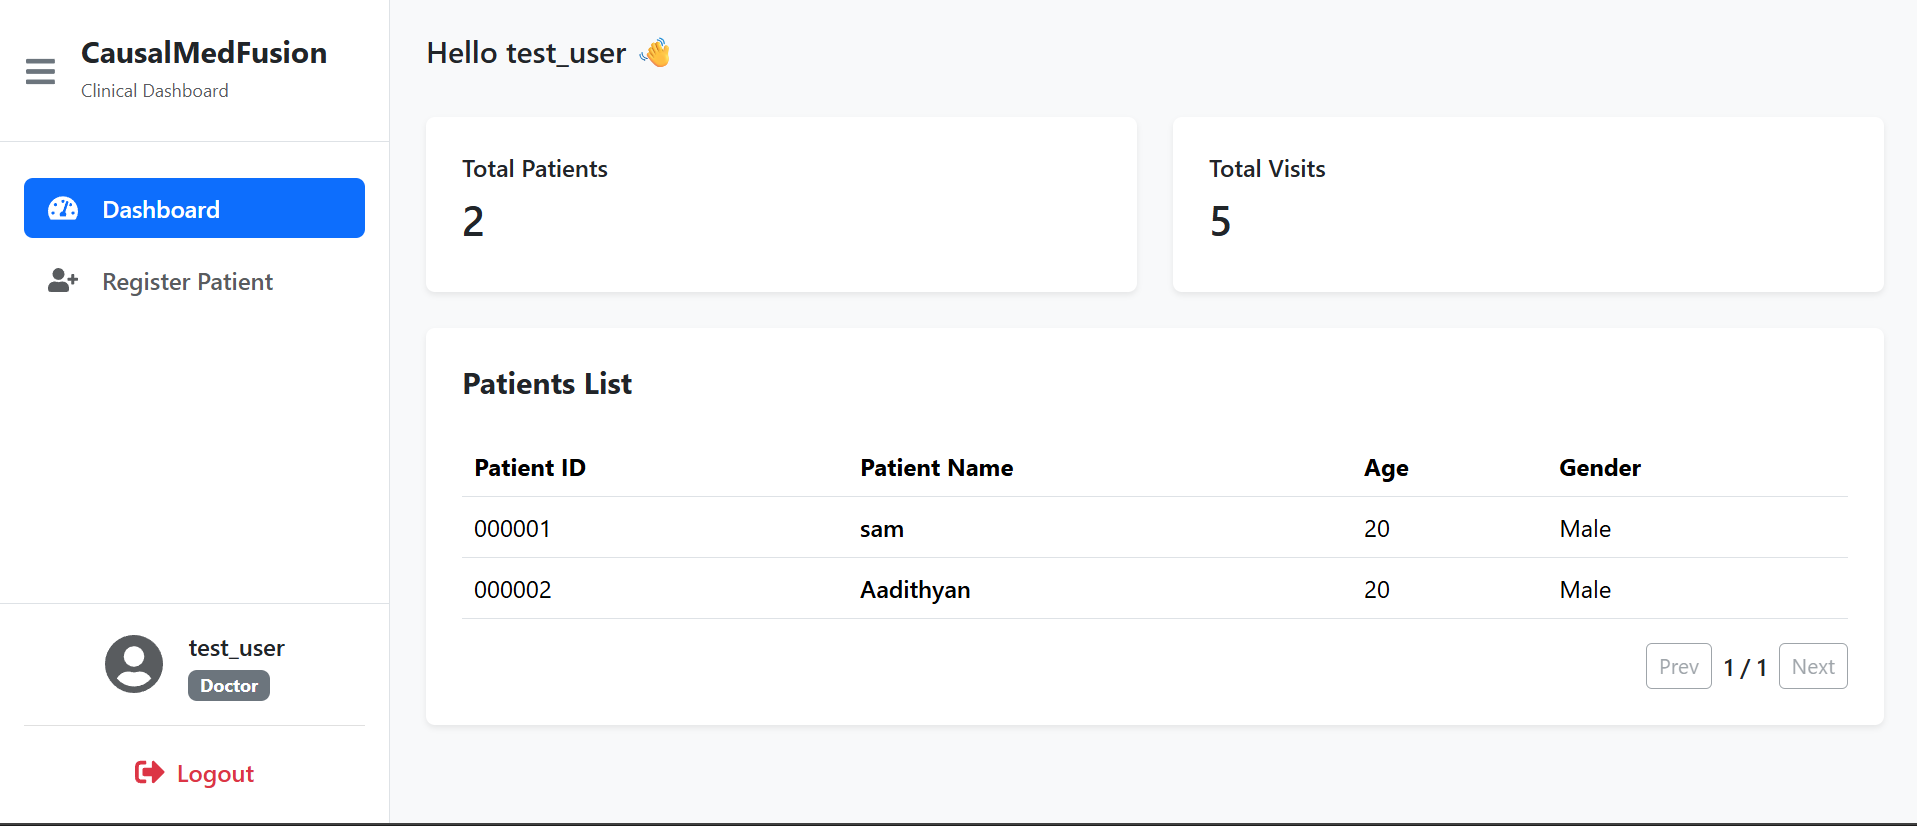
\includegraphics[width=0.9\textwidth]{screenshots/DoctorDashboardPage.png}
    \caption{Clinician's Main Dashboard}
\end{figure}
\noindent \textbf{Description:} Upon logging in, the clinician views this central dashboard listing active assigned patients and high-level health metrics.

\begin{figure}[H]
    \centering
    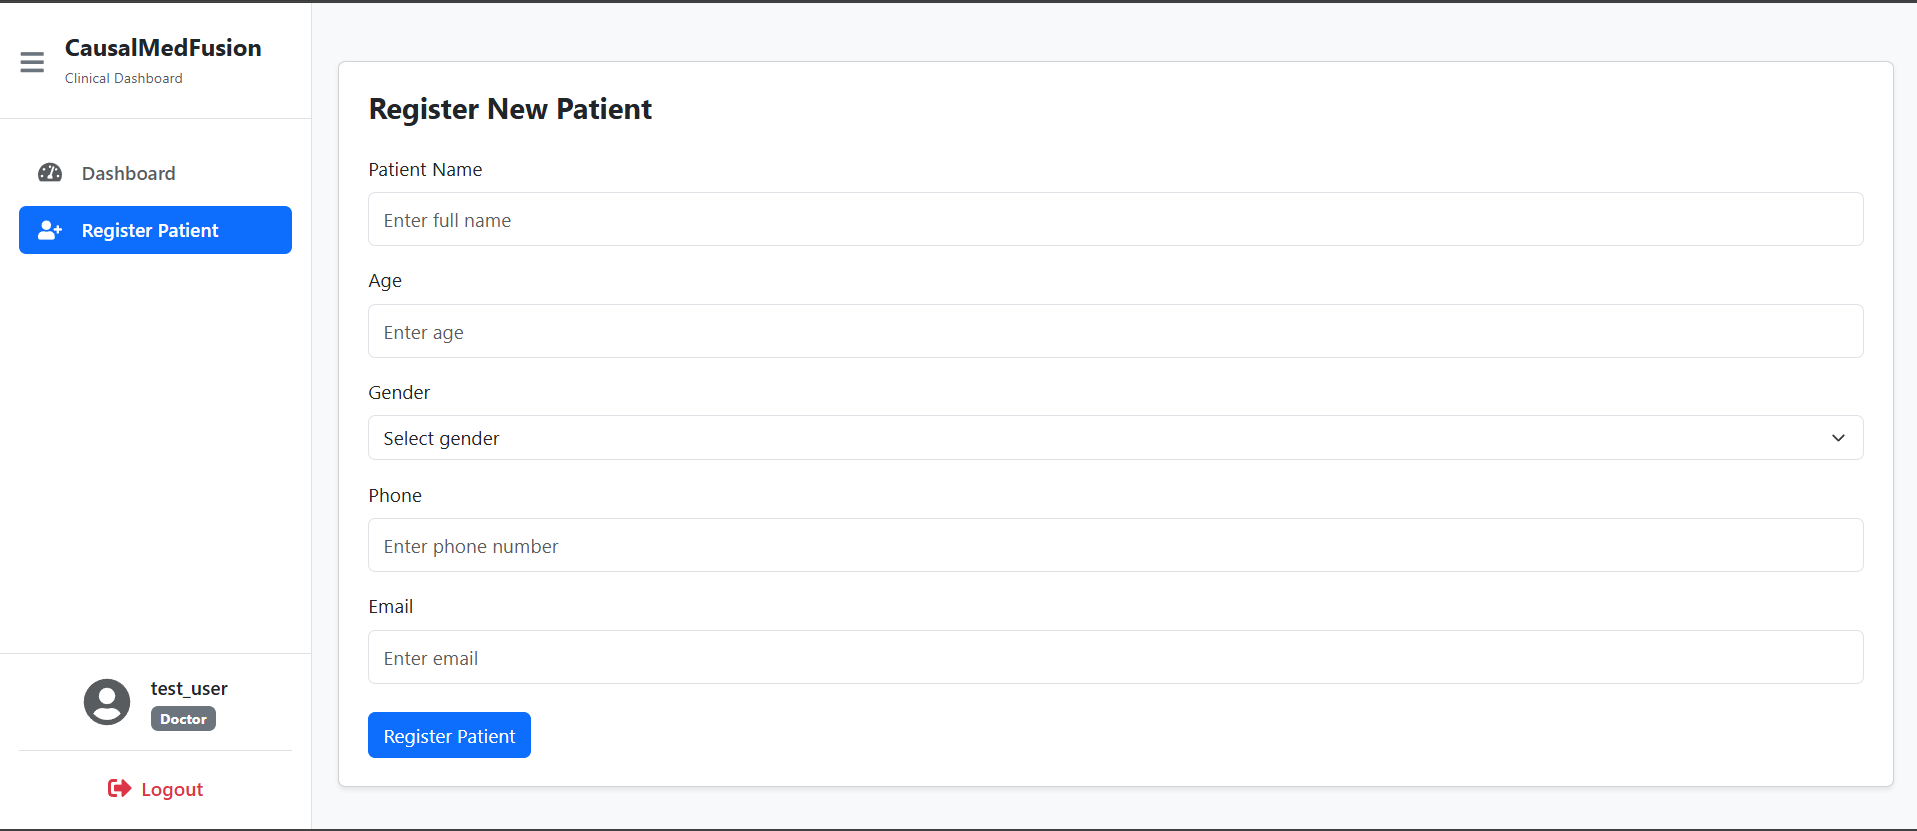
\includegraphics[width=0.9\textwidth]{screenshots/PatientSignupPage.png}
    \caption{Patient Registration Form}
\end{figure}
\noindent \textbf{Description:} A secure interface enabling clinicians to register incoming ICU admissions by capturing discrete patient demographics.

\begin{figure}[H]
    \centering
    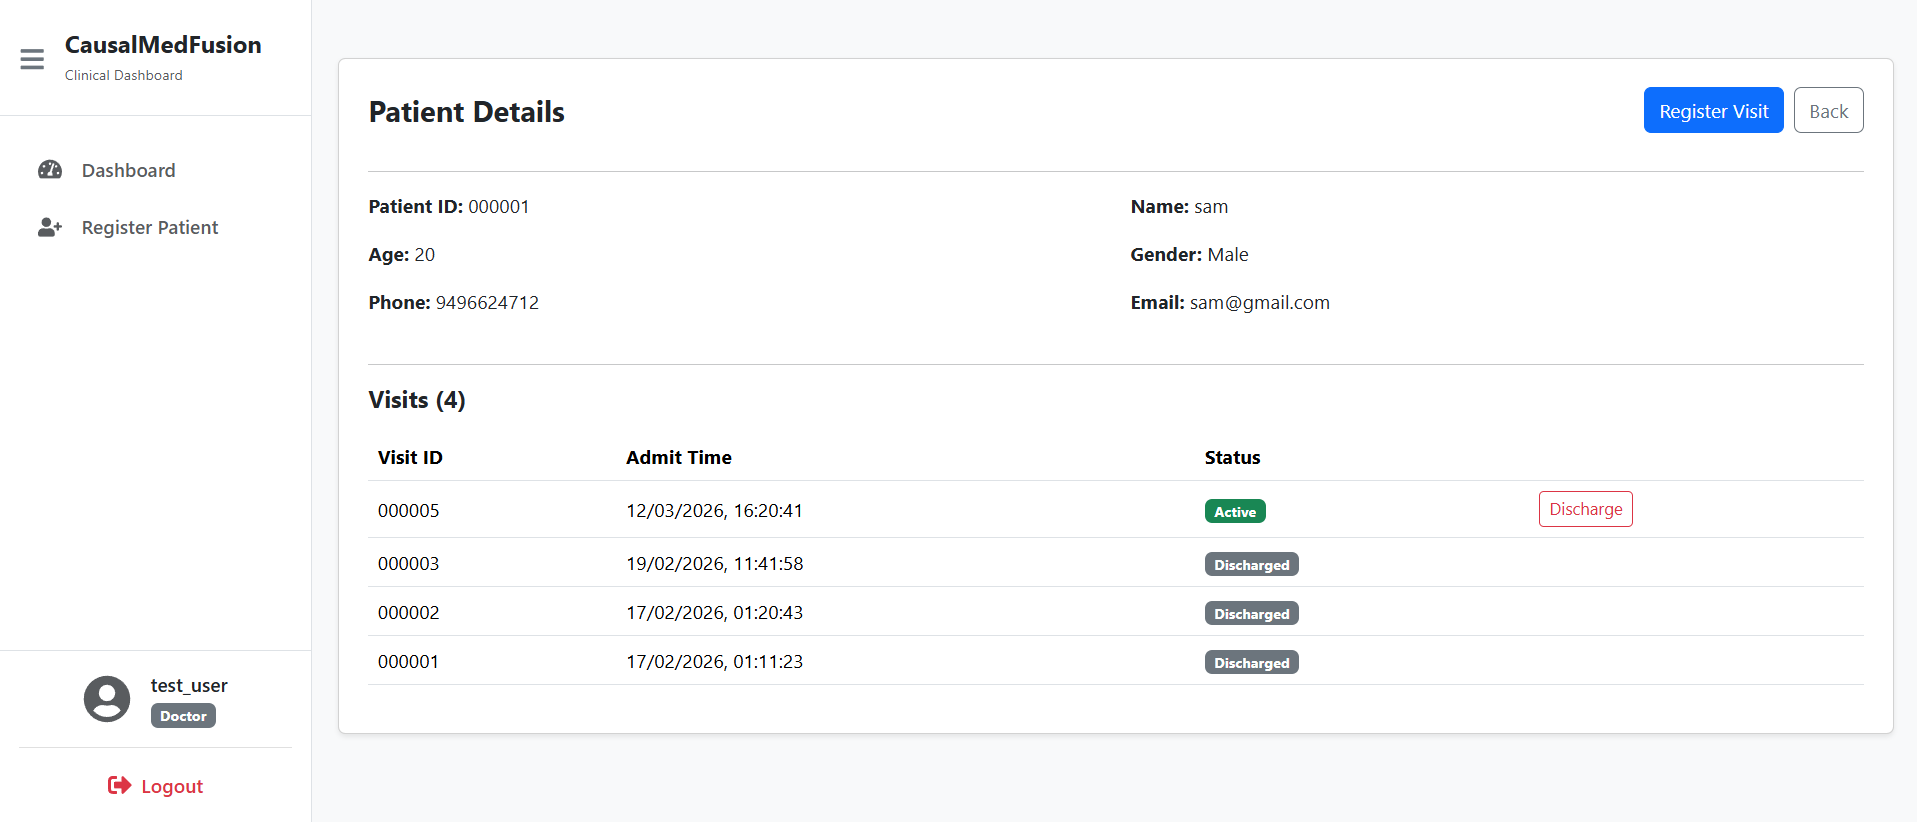
\includegraphics[width=0.9\textwidth]{screenshots/PatientDetailsPage.png}
    \caption{Patient Profile View}
\end{figure}
\noindent \textbf{Description:} This page displays detailed demographic history alongside a chronological log of all previous intensive care visits for the selected patient.

\begin{figure}[H]
    \centering
    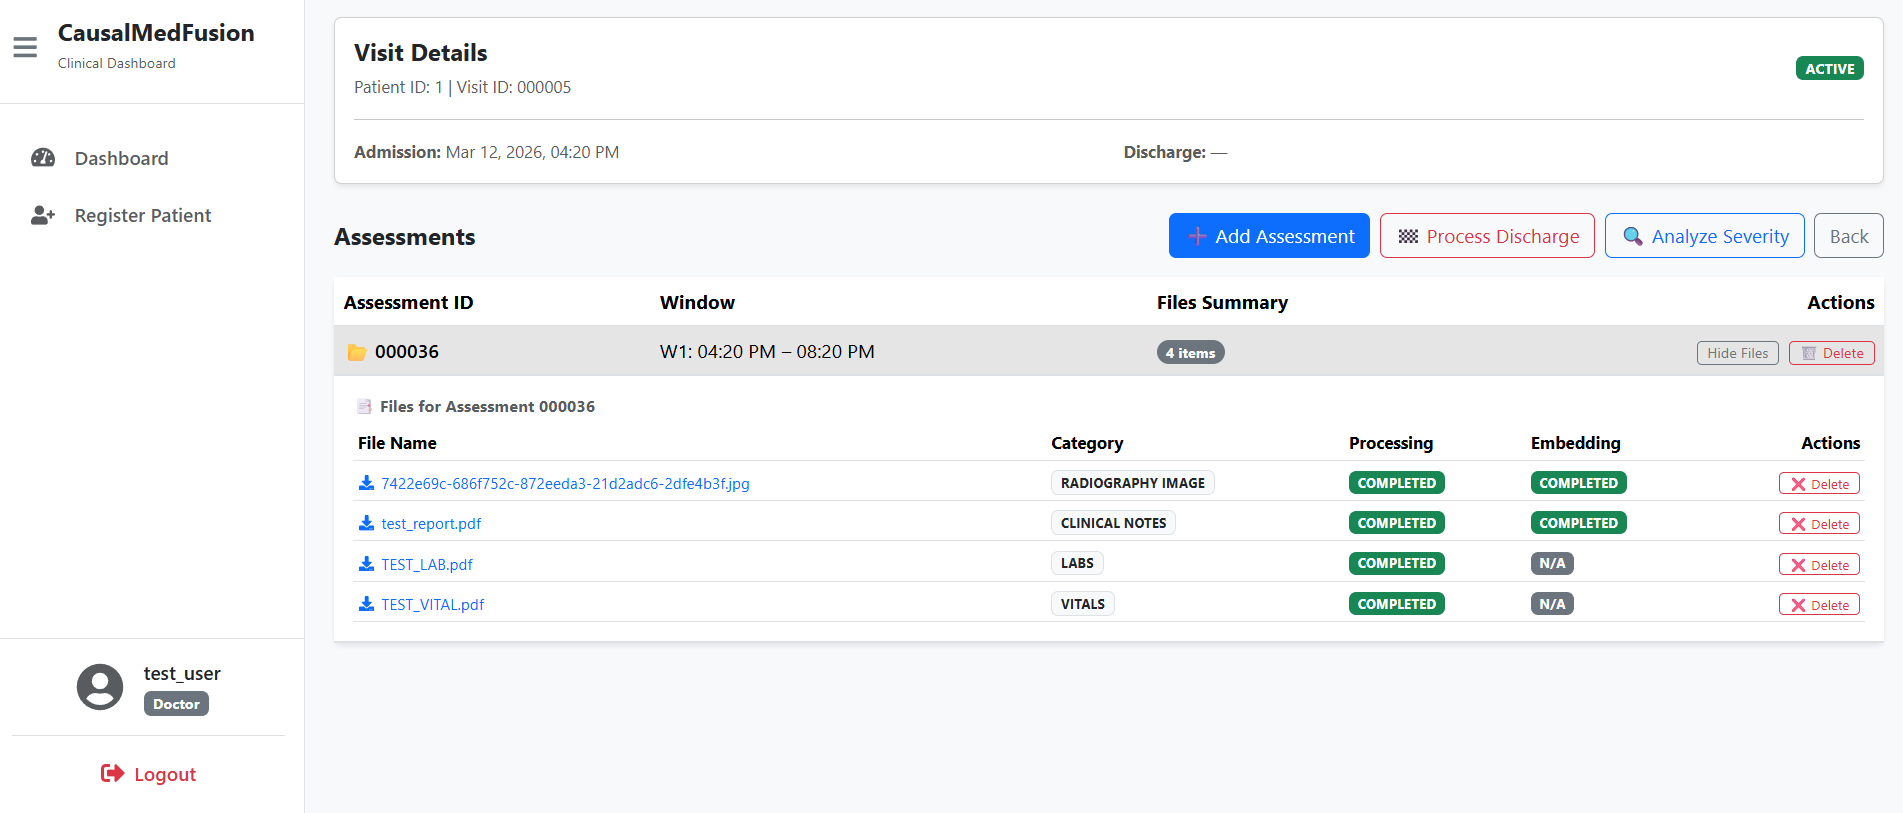
\includegraphics[width=0.9\textwidth]{screenshots/VisitDetailsPage.png}
    \caption{Visit-Level Overview}
\end{figure}
\noindent \textbf{Description:} The Visit Details interface visualizes localized analytics relative to a single continuous ICU stay, tracking individual multimodality assessment states.

\begin{figure}[H]
    \centering
    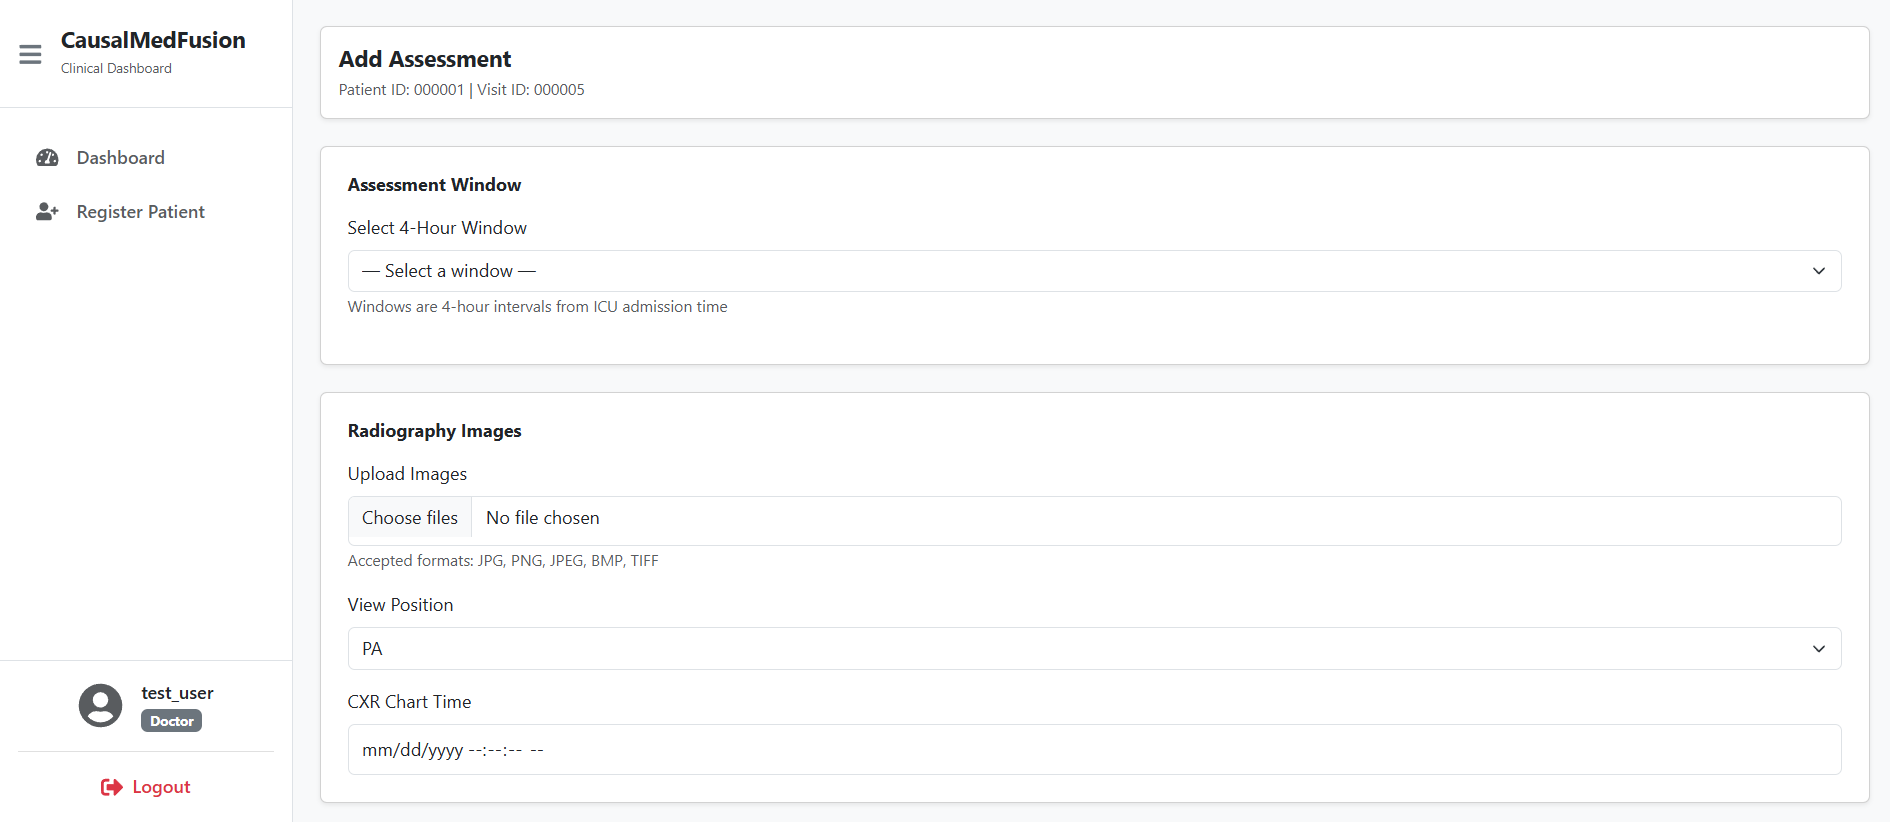
\includegraphics[width=0.9\textwidth]{screenshots/AddAssessmentsPage.png}
    \caption{Multimodal File Uploader}
\end{figure}
\noindent \textbf{Description:} A critical data ingestion pipeline permitting personnel to securely upload asynchronous Chest X-Rays, Clinical Texts, Vitals, and Laboratory CSVs.

\begin{figure}[H]
    \centering
    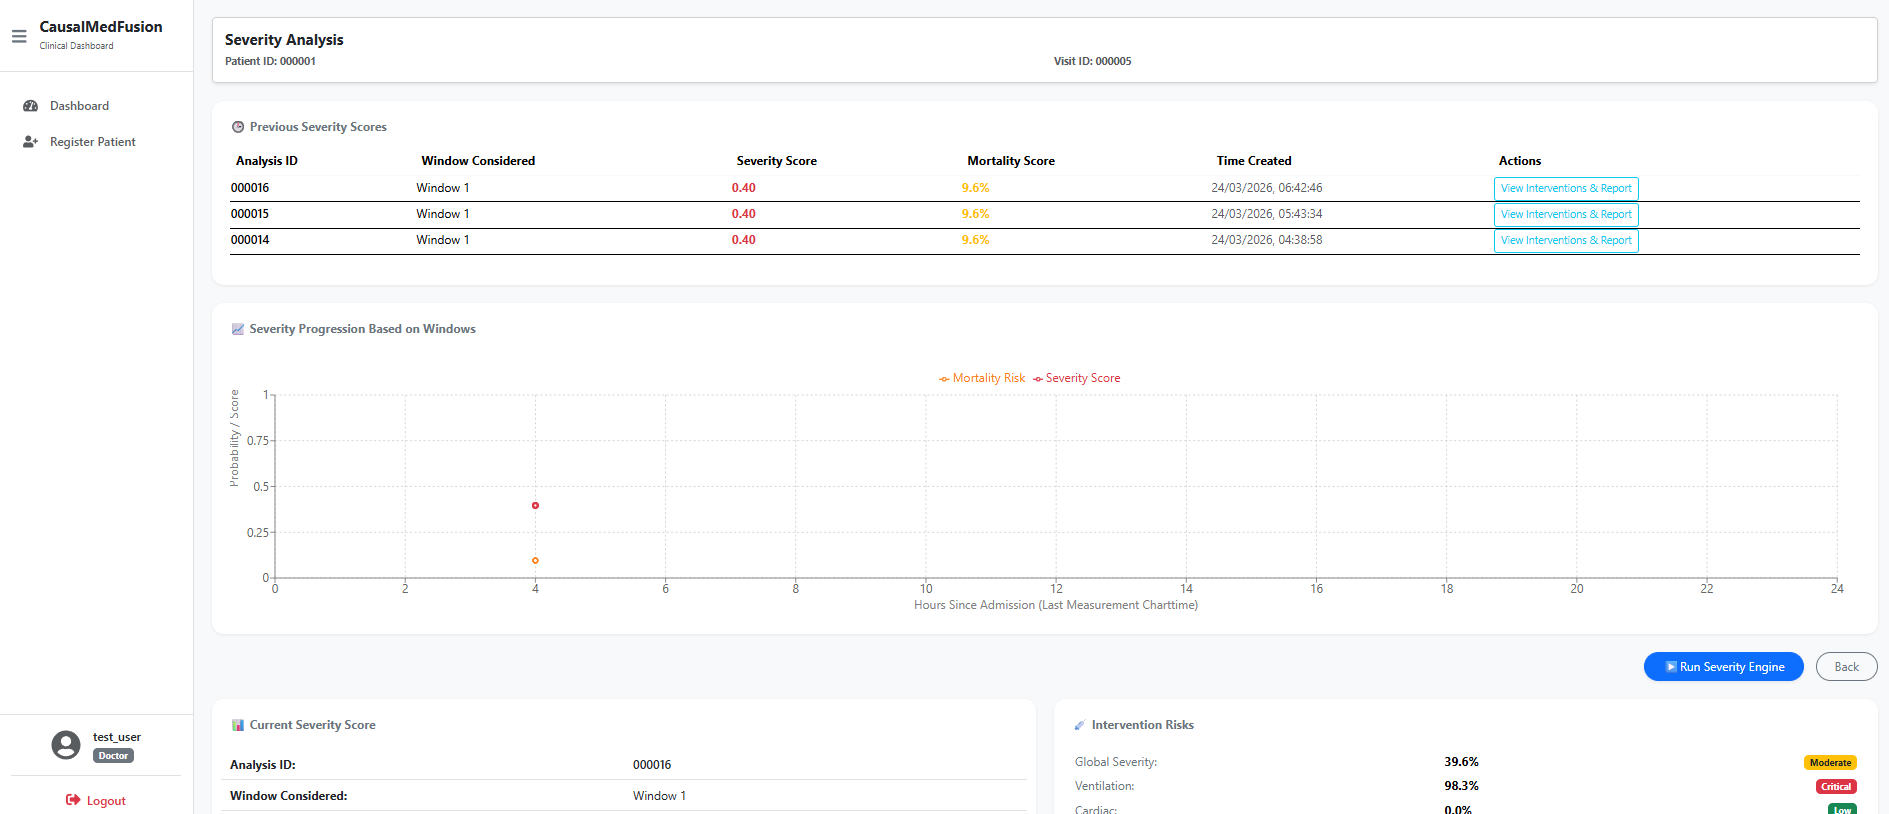
\includegraphics[width=0.9\textwidth]{screenshots/SeverityAnalysisPage.png}
    \caption{Intervention \& Severity Analytics Results}
\end{figure}
\noindent \textbf{Description:} The core inference dashboard showing ML Gateway outputs. It graphs the patient's severity progression over 4-hour aligned windows and renders precise intervention risks (Ventilation, Dialysis, Cardiac Support).

\end{appendices}
\end{document}
